                   
\documentclass[11pt,twoside]{docs/thesis}
%\documentclass[tikz]{standalone}
\usepackage{enumerate}
\usepackage{longtable}
\usepackage{url}
\usepackage{hyperref}
\usepackage{makeidx}
\usepackage{graphics}
\usepackage{multicol}
\usepackage[spanish]{babel}
%\usepackage{translator}


\usepackage{datetime}
\yyyymmdddate
\usepackage{pdflscape} % provides the landscape environment
\usepackage{ragged2e} % provides \RaggedLeft

%%%%%%%%%%%%%%%%
% TITULO DEL PROYECTO
%%%%%%%%%%%%%%%%
%\titulo{T\'itulo del Trabajo de Grado}

\titulo{Diseño de sistema automático de monitoreo alimenticio de bajo costo para productores ganaderos de reses estabuladas en proceso de ceba} 


%%%\titulo{Diseño de sistema automático de monitoreo alimenticio de bajo costo para productores ganaderos de reses estabuladas en proceso de ceba en el municipio de Cajibío - Cauca}


%Para TAMURA: 
%%%%%%%
% AUTOR(ES)
%%%%%%%
%\autorA{COD}{Primer Autor}
\autorA{2117293}{Luis Felipe Guevara Gómez}
%\autorB{COD}{Segundo Autor} %Opcional

%%%%%%%
% FECHA DE ENTREGA
%%%%%%%

\fecha{\today}

%%%%%%%%%%%%%%%%%
% DIRECTOR DEL PROYECTO
% DIRECTOR DE CARRERA
%%%%%%%%%%%%%%%%%

%\directorproyecto{Dr.}{Nombre del Director}
\directorproyecto{Dr.}{Eugenio Tamura Morimitsu}
%\codirectorproyecto{Dr.}{Luis Fernando Macea Mercado}
\directorcarrera{Dr.}{Eugenio Tamura Morimitsu}

\usepackage{amsmath,amssymb}             % AMS Math
% \usepackage[french]{babel}
\usepackage[latin1]{inputenc}
\usepackage[T1]{fontenc}
\usepackage{rotating,amsmath,booktabs,graphicx} % March 2023
\usepackage{xcolor}
\usepackage{caption}
\usepackage{subcaption}
% \usepackage{nomenc1}
\usepackage{paralist}
\usepackage{ulem}
\usepackage{etoolbox}
\usepackage[left=1.0in,right=1.0in,top=1.0in,bottom=1.0in,includefoot,includehead,headheight=13.6pt]{geometry}
\renewcommand{\baselinestretch}{1.05}
%  19/10/19
% \newcommand{\squeezeup}{\vspace{-2.5mm}}
% 19/10/19

% Table of contents for each chapter

\usepackage[nottoc, notlof, notlot]{tocbibind}
\usepackage{minitoc}



%%%%%%%%%%%%%%%%%%%%%%%%%%%%%%%%%%%%%%%%%%%%%%%%%%%%%%%%%%%%%%%%%%%
%%%%%%%%%%%%%%%%%%%%%%%%%%%%%%%%%%%%%%%%%%%%%%%%%%%%%%%%%%%%%%%%%%%

\usepackage{pgfgantt}

\definecolor{darkgreen}{RGB}{0,176,80}
\definecolor{lightgreen}{RGB}{169,208,142}
\definecolor{beige}{RGB}{242,242,242}
\definecolor{blue2}{RGB}{189,215,238}
\definecolor{barblue}{RGB}{153,220,254}
\definecolor{groupblue}{RGB}{51,102,254}
\definecolor{linkred}{RGB}{165,0,33}
\definecolor{groupgreen}{RGB}{0,240,0}
\definecolor{bargreen}{RGB}{0,220,0}
\definecolor{tabla1}{RGB}{255,217,102}
\definecolor{tabla2}{RGB}{189,215,238}

\renewcommand\sfdefault{phv}
\renewcommand\mddefault{mc}
%\renewcommand\bfdefault{bc}
\setganttlinklabel{s-s}{S -> S}
\setganttlinklabel{f-s}{F -> S}
\setganttlinklabel{f-f}{F -> F}
\sffamily

%%
%%
%%\usepackage{datetime}
%%\renewcommand{\dateseparator}{-} 
\yyyymmdddate
%%\today

%%%%%%%%%%%%%%%%%%%%%%%%%%%%%%%%%%%%%%%%%%%%%%%%%%%%%%%%%%%%%%%%%%%
%%%%%%%%%%%%%%%%%%%%%%%%%%%%%%%%%%%%%%%%%%%%%%%%%%%%%%%%%%%%%%%%%%%

\setcounter{minitocdepth}{2}
\mtcindent=15pt
% Use \minitoc where to put a table of contents

\usepackage{aecompl}
\usepackage{adjustbox}

% My pdf code

\usepackage{ifpdf}


% Links in pdf
\usepackage{color}
\definecolor{linkcol}{rgb}{0,0,0.4} 
\definecolor{citecol}{rgb}{0.5,0,0} 

% Change this to change the informations included in the pdf file

% See hyperref documentation for information on those parameters

\hypersetup
{
bookmarksopen=true,
pdftitle="Prototipo semi-automático para monitoreo alimenticio de reses estabuladas en proceso de ceba",
pdfauthor="Luis Felipe Guevara Gómez", 
pdfsubject="Trabajo de Grado | Ingeniería Electrónica | Javeriana Cali", %subject of the document
%pdftoolbar=false, % toolbar hidden
pdfmenubar=true, %menubar shown
pdfhighlight=/O, %effect of clicking on a link
colorlinks=true, %couleurs sur les liens hypertextes
pdfpagemode=None, %aucun mode de page
pdfpagelayout=SinglePage, %ouverture en simple page
pdffitwindow=true, %pages ouvertes entierement dans toute la fenetre
linkcolor=linkcol, %couleur des liens hypertextes internes
citecolor=citecol, %couleur des liens pour les citations
urlcolor=linkcol %couleur des liens pour les url
}

% definitions.
% -------------------

\setcounter{secnumdepth}{3}
\setcounter{tocdepth}{2}

% Some useful commands and shortcut for maths:  partial derivative and stuff

\newcommand{\pd}[2]{\frac{\partial #1}{\partial #2}}
\def\abs{\operatorname{abs}}
\def\argmax{\operatornamewithlimits{arg\,max}}
\def\argmin{\operatornamewithlimits{arg\,min}}
\def\diag{\operatorname{Diag}}
\newcommand{\eqRef}[1]{(\ref{#1})}

\usepackage{rotating}                    % Sideways of figures & tables
%\usepackage{bibunits}
%\usepackage[sectionbib]{chapterbib}          % Cross-reference package (Natural BiB)
\usepackage{natbib}                  % Put References at the end of each chapter
    % Do not put 'sectionbib' option here.
    % Sectionbib option in 'natbib' will do.
\usepackage{fancyhdr}                    % Fancy Header and Footer

% \usepackage{txfonts}                     % Public Times New Roman text & math font
  
%%% Fancy Header %%%%%%%%%%%%%%%%%%%%%%%%%%%%%%%%%%%%%%%%%%%%%%%%%%%%%%%%%%%%%%%%%%
% Fancy Header Style Options

\pagestyle{fancy}                       % Sets fancy header and footer
\fancyfoot{}                            % Delete current footer settings

%\renewcommand{\chaptermark}[1]{         % Lower Case Chapter marker style
%  \markboth{\chaptername\ \thechapter.\ #1}}{}} %

%\renewcommand{\sectionmark}[1]{         % Lower case Section marker style
%  \markright{\thesection.\ #1}}         %

\fancyhead[LE,RO]{\bfseries\thepage}    % Page number (boldface) in left on even
% pages and right on odd pages
\fancyhead[RE]{\bfseries\nouppercase{\leftmark}}      % Chapter in the right on even pages
\fancyhead[LO]{\bfseries\nouppercase{\rightmark}}     % Section in the left on odd pages

\let\headruleORIG\headrule
\renewcommand{\headrule}{\color{black} \headruleORIG}
\renewcommand{\headrulewidth}{1.0pt}
\usepackage{colortbl}
\arrayrulecolor{black}

\fancypagestyle{plain}{
  \fancyhead{}
  \fancyfoot{}
  \renewcommand{\headrulewidth}{0pt}
}

\usepackage{algorithm}
\usepackage[noend]{algorithmic}

%%% Clear Header %%%%%%%%%%%%%%%%%%%%%%%%%%%%%%%%%%%%%%%%%%%%%%%%%%%%%%%%%%%%%%%%%%
% Clear Header Style on the Last Empty Odd pages
\makeatletter

\def\cleardoublepage{\clearpage\if@twoside \ifodd\c@page\else%
  \hbox{}%
  \thispagestyle{empty}%              % Empty header styles
  \newpage%
  \if@twocolumn\hbox{}\newpage\fi\fi\fi}

\makeatother
 
%%%%%%%%%%%%%%%%%%%%%%%%%%%%%%%%%%%%%%%%%%%%%%%%%%%%%%%%%%%%%%%%%%%%%%%%%%%%%%% 
% Prints your review date and 'Draft Version' (From Josullvn, CS, CMU)
\newcommand{\reviewtimetoday}[2]{\special{!userdict begin
    /bop-hook{gsave 20 710 translate 45 rotate 0.8 setgray
      /Times-Roman findfont 12 scalefont setfont 0 0   moveto (#1) show
      0 -12 moveto (#2) show grestore}def end}}
% You can turn on or off this option.
% \reviewtimetoday{\today}{Draft Version}
%%%%%%%%%%%%%%%%%%%%%%%%%%%%%%%%%%%%%%%%%%%%%%%%%%%%%%%%%%%%%%%%%%%%%%%%%%%%%%% 

\newenvironment{maxime}[1]
{
\vspace*{0cm}
\hfill
\begin{minipage}{0.5\textwidth}%
%\rule[0.5ex]{\textwidth}{0.1mm}\\%
\hrulefill $\:$ {\bf #1}\\
%\vspace*{-0.25cm}
\it 
}%
{%

\hrulefill
\vspace*{0.5cm}%
\end{minipage}
}

\let\minitocORIG\minitoc
\renewcommand{\minitoc}{\minitocORIG \vspace{1.5em}}

\usepackage{multirow}
%\usepackage{slashbox}

\newenvironment{bulletList}%
{ \begin{list}%
	{$\bullet$}%
	{\setlength{\labelwidth}{25pt}%
	 \setlength{\leftmargin}{30pt}%
	 \setlength{\itemsep}{\parsep}}}%
{ \end{list} }

\renewcommand{\epsilon}{\varepsilon}

% centered page environment

\newenvironment{vcenterpage}
{\newpage\vspace*{\fill}\fancyhf{}\renewcommand{\headrulewidth}{0pt}}
{\vspace*{\fill}\par\pagebreak}

\makeindex



\begin{document}

%\renewcommand{\dateseparator}{-} 
%\yyyymmdddate
%\today
\maketitle
\makecoverletter

%%%%%%%%%%%%%%%%%%
% ABSTRACT
%%%%%%%%%%%%%%%%%%
\chapter*{Agradecimientos} %%%%%%%%%%%%%%%%%%%%%
%% AGRADECIMIENTOS %%
%%%%%%%%%%%%%%%%%%%%%

Quiero agradecer a mi director de proyecto, el \director, por su guía, conocimiento, paciencia  y apoyo en la finalización de este proyecto. También agradecer al  equipo del Centro Agropecuario del Servicio Nacional de Aprendizaje, seccional Popayán (CA-SENA-POP) por brindarme su apoyo, experticia y confianza al suministrarme los datos y la información necesaria para realizar mi proyecto.\\

A mis familiares y amigos por su presencia y apoyo moral.\\ 

Y sobre todo, especial dedicatoria a mis padres, hermanos y abuelos, por inspirarme, alentarme, apoyarme y siempre darme ánimos y fuerza para seguir adelante en la búsqueda de mis sueños y mi futuro.\\



\chapter*{Glosario} %%%\subsection{Definici\'on de t\'erminos}
%Para el correcto entendimiento de este proyecto es necesario aclarar la definici\'on de los siguientes t\'erminos:\\
% 
%\begin{itemize}
%
%	\item \textbf{Algoritmo:} Conjunto ordenado y finito de operaciones que permite hallar la solución de un problema. \cite{defalgoritmo}.
%	
%	
%	%Estos novillos experimentan la ceba entre sus 18 a 24 meses o hasta que obtienen un peso  deseado entre los 450 y 500 kg.
%	
%	
%	
%		
%		
%\end{itemize}
\chapter*{Resumen}  %%%%%%%%%%%%%%%%%%%%%%%%%%%%%
% RESUMEN <==>  ABSTRACT	%
%%%%%%%%%%%%%%%%%%%%%%%%%%%%%
%Resumen de la propuesta. (1/2 página). \\
Modelar dinámicamente un sistema es importante para representar de manera simplificada su comportamiento sin recurrir a la experimentación, que para sistemas complejos, puede representar un alto consumo de recursos. También es útil para predecir comportamientos a largo plazo; observar, analizar, e interpretar resultados, frente a diferentes entradas que afectan directa o indirectamente a el o los subsistemas presentes; establecer conclusiones y apoyar la toma de decisiones futuras.\\
% 

Este trabajo estudia el comportamiento productivo de ganado bovino y bufalino del Centro Agropecuario del Servicio Nacional de Aprendizaje (SENA), ubicado en la ciudad de Popayán (CA-SENA-POP); teniendo en consideración diferentes variables; entre ellas, la producción de leche, el consumo de agua, consumo de forrajes, consumo de concentrado, generación de desperdicios y finalmente utilidades por venta de producciones de leche y ganado para carne. El objetivo es estructurar y evaluar un modelo basado en ecuaciones diferenciales que facilite observar respuestas del sistema productor ganadero ante diferentes entradas, en pro de predecir comportamientos a largo plazo.\\

Este proyecto adapta de manera flexible la metodología CRISP-DM, con la que se busca ajustar conjuntos de datos a curvas lineales y no lineales, de tal forma que se proceda a modelar dinámicamente las respuestas del sistema productor ganadero frente a diferentes entradas. Este proyecto también utiliza conjuntos de datos debidamente registrados y proveídos por el SENA tanto de manera análoga como digital. Los resultados obtenidos son necesarios para prever situaciones futuras y evaluar el rendimiento del modelo frente a nuevos datos.\\

{\bf Palabras y Conceptos Clave}: Ajuste de curvas, Modelamiento Dinámico, Producción ganadera.
\chapter*{Abstract} %%%%%%%%%%%%%%%%%%%%%%%%%%%%%
% RESUMEN <==>  ABSTRACT	%
%%%%%%%%%%%%%%%%%%%%%%%%%%%%%
%Resumen de la propuesta. (1/2 página). \\

Modeling a system dynamically is important to represent its behaviour in a simplified way without resorting to experimentation, which for complex systems, it could represent a high resource consumption. It is also useful to predict long term responses; observe, analyze and interpret results against different inputs that directly or indirectly affect subsystem(s) present; draw conclusions and support future decision making.\\

This work studies the functioning of livestock production in the Agricultural Center of the National Apprenticeship Service, Popayan sectional (CA-SENA-POP); taking into account a variety of variables such as milk yield; water, fodder and concentrated food consumption; waste generation and last but not least, profit from milk and meat production sales. The objective is to structure and assess a model based on differential equations that facilitates the visualization of the CA-SENA-POP livestock system against different situations for long term behaviour prediction.\\

This project adapts, in a felixible way, the CRISP-DM methodology, with which it is sought to adjust
data sets to linear and nonlinear curves in such a way that the responses of the livestock production system to different inputs are dynamically modeled. This project also uses properly registered and organized databases provided by the SENA institution,both analog and digital.
The results obtained are necessary to foresee future situations and evaluate the performance of the model against new data.\\


{\bf Keywords}: Curve fitting, Dynamic modeling, Livestock production.


%%%%%%%%%%%%%%%%%
%%%% TABLE OF CONTENTS
%%%% AND PREABLE
%%%%%%%%%%%%%%%%%
  
  
\tableofcontents  % ==================>    ESTE ES EL INDICE GENERAL     <=======================
\listoffigures 	  % ==================>    ESTE ES EL INDICE DE FIGURAS  <=======================
\listoftables     % ==================>    ESTE ES EL INDICE DE TABLAS   <=======================
\mainmatter       % ==================>    ESTE NO SE QUE ES...     <=======================


\dominitoc
\cleardoublepage

%%%%%%%%%%%%%%%%%%%%%%
% INTRODUCCION
%%%%%%%%%%%%%%%%%%%%%%
\chapter{Introducci\'on}

%%%%%%%%%%%%%%%%%%%%
% INTRODUCCION
%%%%%%%%%%%%%%%%%%%%
%%Introducción general al problema que se va a resolver. (1 %%página)
%%%%\begin{align*}
%%%%\sin(x)=e^{2 \pi \theta \widehat{g}}\\
%%%%\sin(x)=e^{2 \pi}+\sin(x)
%%%%\end{align*}

En los últimos años, el sector agropecuario ha ido retomando gran importancia en Latinoamérica y el mundo, debido a múltiples factores entre los cuales se puede resaltar el crecimiento poblacional, que lleva consigo el incremento del consumo de alimentos. Esto representa una necesidad que puede y debe ser resuelta con el crecimiento de la producción agropecuaria de hasta un 70\% para satisfacer la demanda alimenticia a nivel mundial. Para ello es de vital importancia que los países en desarrollo como Colombia, entren a formar parte del mercado altamente productivo y competitivo haciendo uso de las fuentes que le aportan una ventaja comparativa en la región que radican, siendo estas la abundancia de recursos hidrícos y terrestres \cite{fao}.\\

Actualmente, Brasil es el segundo mayor proveedor de alimentos y productos agropecuarios a nivel mundial y cuenta con mejoras continuas en los procesos de producción, que respaldan el rápido crecimiento de las exportaciones. La investigación agropecuaria ha sido uno de los factores clave para el incremento de la productividad en la región durante las últimas décadas, con el fin de hacer seguimiento al registro, tratamiento, manipulación y analisis  los datos y el desempeño de los sistemas de investigación y desarrollo agropecuario mediante la evaluación de resultados. Estos datos son una herramienta indispensable cuando se trata de evaluar el aporte de la I+D agropecuaria y de manera más general, el crecimiento económico de la región y el país.\\

En America Latina y más precisamente en Colombia, sobresale la formación de 55 Comités de Investigación Agricola elegidos Localmente (CIAL). Estos están constituidos por agricultores experimentados que administran y conducen investigación y desarrollo en beneficio de toda la comunidad \cite{ashby}; así pues se representa la alta participación colombiana en este ámbito de desarrollo.

En Colombia también se han incorporado nuevas entidades que aportan al desarrollo investigativo, productivo y competitivo como la Corporación Colombiana de Investigación Agropecuaria (AGROSIVA), que de mano con la expedición de la Ley 1876 de 2017 donde se crea el Sistema Nacional de Innovación Agropecuaria (SNIA), buscan integrar la ciencia, y el desarrollo tecnológico del sector junto con la formación y prestación del servicio de extensión agropecuaria. En este sentido, la ciencia permite lograr avances en términos productivos, de innovación y de competitividad \cite{minagricultura}.\\

En el Cauca, de acuerdo con el Instituto Geográfico Agustín Codazzi, los suelos del departamento presentan casi todos los pisos térmicos de variadas fertilidades y profundidades, y con diversas vocaciones para su uso \cite{igac}. Por otra parte, aunque comúnmente pueda considerarse un sector primitivo o de poca inversión tecnológica, el sector agropecuario cuenta con el mayor potencial tecnológico para el desarrollo sostenible y es uno de los más tecnificados en la región. Esto debido a la inclusión de nuevas tecnologías, no solo para la ejecución de procesos, sino también para la gestión y el manejo de las grandes cantidades de datos, impulsando así, el desarrollo competitivo del campesino e incrementando su participación en el mercado a nivel regional, nacional y mundial.

No obstante, la inclusión de las actuales tecnologías puede significar una gran inversión económica para pequeños y medianos productores y cultivadores. Los altos costos significan un impedimento a la participación competitiva en el mercado ganadero y de cultivos varios, con lo que el mejoramiento de pequeñas partes del sistema total puede manifestarse en mejoras significativas en el día a día de los nuevos emprendedores ganaderos. Estos costos se pueden taxonomizar en costos de producción, mantenimiento, transporte, control, toma, registro, seguimiento, manipulación y representación de datos; que diariamente aportan al consumo de recursos limitados como los económicos, personales y tiempo. Para ello se requiere de nuevos enfoques que permitan mejorar algunas de las condiciones de trabajo de los cultivadores agrícolas promoviendo la integración científica, innovadora y competitiva.\\

Con base en todo lo anterior, se considera indispensable la inclusión de tecnologías y metodologías de tratamiento, simulación y modelamiento computacional de los datos presentes en la producción ganadera.

%%%%%%%%%%%%%%%%%%%%%%
% DESCRIPCION DEL PROBLEMA
%%%%%%%%%%%%%%%%%%%%%%

\section{Planteamiento del Problema}

El sector ganadero abarca diferentes especies de ganado tales como los bovinos, los ovinos, bufalinos, entre otros. En Colombia se tiene una alta presencia de producción de estos tipos especialmente en el ganado bovino y ovino. De igual forma, estos tipos de ganado tienen diferentes modalidades, entre las que se pueden mencionar el ganado para crianza, para producción de leche y sus derivados, y ganadería de la carne o doble propósito. En Colombia y el mundo se presentan constantes inversiones en materia tecnológica y metodológica para mejorar la forma en cómo el ganado es productivo y puede participar de forma competitiva en un mercado de consumo de calidad \cite{fao}.\\

Aunque en el Cauca se cuente con vastas hectáreas de diferentes fertilidades y condiciones térmicas apropiadas para el cultivo y desarrollo de la ganadería \cite{igac}, aún se presentan falencias en materia de inversión tecnológica, económica e investigativa, en donde los movimientos migratorios de campesinos desplazados y los efectos colaterales del conflicto armado que se ha presentado en el país, son las principales causas de estas falencias \cite{fao}.Sin embargo, el emprendimiento de los pequeños y medianos productores da paso a nuevas oportunidades de intervención por parte de la ingeniería, modelamiento matemático e inclusión de metodologías de análisis, clasificación, tratamiento y manejo cuantitativo de datos por medios como la Inteligencia Artificial. \\

El manejo de software sofisticado, métodos o modelos matemáticos; pueden presuponer brechas para los productores campesinos por la falta de capacitación técnica, o por la complejidad de uso de los programas para el manejo, análisis y procesamiento de datos, lo que resulta en que la toma de decisiones dependa de un enfoque tradicional, mas no sistémico.\\

A pesar de ello, en el último siglo, la investigación a nivel global ha posibilitado la estimación del comportamiento de variables asociadas a la producciones agropecuarias tales como la leche, la carne, y el consumo de insumos, a través de modelos matemáticos que varían en complejidades lineales o no lineales como se menciona en \cite{lechepaisa1}, \cite{caprinos}, \cite{colombiaherd}. Adicionalmente a esto, en las últimas décadas se han desarrollado múltiples investigaciones en las que, computacional mente se modelan sistemas dinámicos de producción lechera tales como \cite{janaina1}, \cite{janaina2}, \cite{hdmwallace}, \cite{avila1}; lo que presupone una herramienta de ayuda para apoyar la toma de decisiones en los sistemas de producción ganadera \cite{gavira}.\\

% En la ganadería lechera, se maneja el término de curvas de lactancia, 
% \pagebreak
Tal y como lo mencionan en \cite{minagricultura}, \cite{ashby} y \cite{fao}; la inclusión de las ciencias y la formación de entidades de apoyo al sector agrario pueden aportar significativamente al desempeño de los  cultivos ganaderos. En Colombia, se han realizado estudios investigativos con ganado bovino y caprino en diferentes regiones del país de las que se pueden mencionar \cite{lechepaisa1}, \cite{lechepaisa2}, \cite{lechepastusa}; por lo que se busca posibilitar un desarrollo investigativo similar en producciones ganaderas del departamento del Cauca; tomando como referencia la producción ganadera tecnificada del Servicio Nacional de Aprendizaje (SENA) ubicada en el municipio de Popayán.\\

Con base en lo anterior se plantea un modelamiento dinámico de producción ganadera en el Centro Agropecuario (CA) del Servicio Nacional de Aprendizaje (SENA) ubicado en el municipio de Popayán, con la finalidad de estimar consumos, producciones, y ganancias ganaderas; que sirvan de apoyo en la toma de decisiones futuras del productor.

\chapter{Visión global del sistema}

%%%%%%%%%%%%%%%%%%%%%%
% DESCRIPCION DEL PROBLEMA
%%%%%%%%%%%%%%%%%%%%%%

En este capítulo se describe parte del contexto ganadero actual de cárnicos en Colombia y el Cauca y algunas de las características principales relacionadas al proceso de ceba en ganado vacuno. Estos temas sirven como base conceptual para comprender el análisis y diseño empleados en este proyecto.

%En este capitulo se explica el contexto ganadero actual y algunas de las características principales relacionadas al proceso de ceba.(Esto estaba antes del 15 de Agsoto de 2019 que hice los cambios en bOSCH)

%El titulo debe ser algo como Contexto general de la ganaderia de carne

%Tengo que agregar algo como otro capitulo de solo lo del tornillo (creo que alcanza) o sino agregarlo a lo de ELECTRÜONICA EN EL AGRO y combinar ese capitulo y PONERLE OTRO NOMBRE.


\section{Generalidades agropecuarias} \label{tgan}
%\section{Visión global} \label{tgan}
%\section{Contexto ganadero en Colombia} \label{tgan}

%ESTO SE BORRA-> Explicar el CONTEXTO, síntomas y causas del problema a resolver. (1.5 páginas).EXPLICAR QUE VOY A HACER \\ \\

La fortaleza principal del sector primario colombiano radica en la producción de recursos de la naturaleza. Esto se refiere a las actividades económicas en relación a los procesos de producción en el sector agropecuario. Este sector abarca el conjunto de técnicas y las acciones que permiten trabajar y cultivar la tierra para producir materias primas así como también la producción de recursos de la ganadería.

Por su parte, el sector ganadero alude a los diferentes tipos de ganado de una zona y a las actividades que se emplean para criar y comercializar a estos animales y a los productos derivados de estos. En Colombia se practican diferentes modalidades de ganadería con base en el tipo de ganado de enfoque tales como:

\begin{itemize}
\item Bovinos ó Vacunos
\item Equinos
\item Mulares y asnales
\item Ovinos
\item Porcinos
\end{itemize}

De igual forma, estos tipos de ganado son trabajados con diferentes designaciones, entre las cuales se pueden mencionar:

\begin{itemize}
\item Crianza y material reproductivo: Tiene como objetivo la reproducción de ganado mediante el cruce de individuos con las mejores características biológicas para mejorar así la genética de los individuos. Los mejores ejemplares son comercializados como material reproductivo y producción de leche dependiendo de su sexo (macho y hembra respectivamente), y los demás ejemplares pasan a ser parte de la ganadería de la carne.
\item Producción de leche y derivados lácteos: Como su nombre lo indica, es el ganado designado para la producción cuantitativa y cualitativa de leche mediante ordeño manual, mecánico o eléctrico.
\item Producción de carne: Encaminado a la producción cuantitativa y cualitativa de carne.
\end{itemize}

\subsection{Caracteres zootécnicos del ganado vacuno}

La destinación del ganado vacuno para producción de leche, material reproductivo o engorde depende de algunos factores fisonómicos y biológicos. Por ello se hace mención de estos atributos a continuación:

\begin{figure}[H]
 \begin{center}
 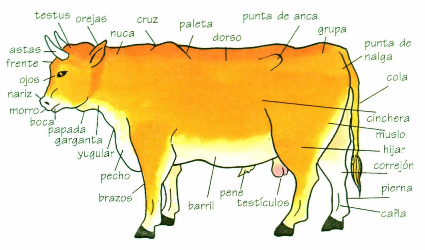
\includegraphics[scale=0.9]{img/dibujito1.png}
 \end{center}
 \caption{Partes físicas de un bovino. Tomada de \cite{librito1}}
\end{figure}

%%% Tek: faltan lsa refs para las figs

\subsubsection{Clasificación vacuna por aptitud productiva}
\begin{itemize}
\item \textbf{Lechero:} (Cabe resaltar que un requerimiento o propiedad fisonómica básica es que posean ubre, esto quiere decir solo las hembras pueden hacer parte de esta aptitud productiva). Poseen formación triangular, cuentan con cuerpo y extremidades largas y delgadas con poca voluminosidad cárnica
\begin{figure}[H]
 \begin{center}
 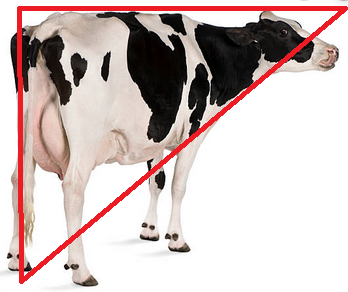
\includegraphics[scale=0.9]{img/dibujito2.png}
 \end{center}
 \caption{Aptitud lechera. Tomada de \cite{googlepics}. }
\end{figure}
\item \textbf{Carne:} Poseen una contextura rectangular. Además de poseer un cuerpo ancho con sus extremidades bien dotadas de carne.
\begin{figure}[H]
 \begin{center}
 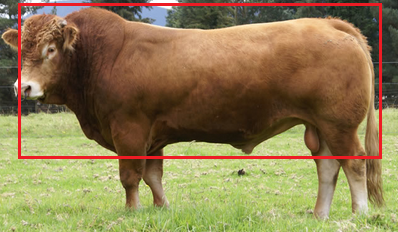
\includegraphics[scale=0.9]{img/dibujito3.png}
 \end{center}
 \caption{Aptitud de tipo carne. Tomada de \cite{googlepics}. }
\end{figure}
\item \textbf{Doble propósito:} Cuentan con propiedades mixtas de los 2 tipos ya mencionados, por lo que tanto su contextura, como volumen cárnico, ubre y extremidades son medianas. Este tipo de animales poseen una mayor facilidad en la adaptación del clima, alimentación y manejo. 
\begin{figure}[H]
 \begin{center}
 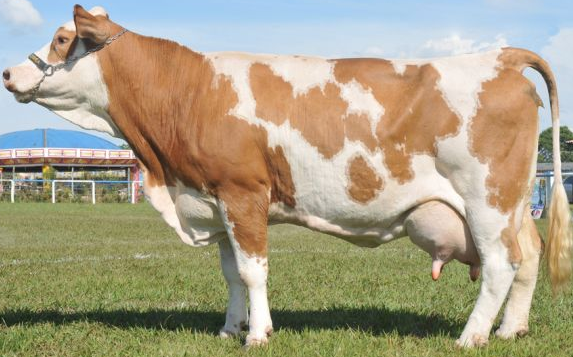
\includegraphics[scale=0.8]{img/dibujito4.png}
 \end{center}
 \caption{Aptitud de doble propósito.  Tomada de \cite{googlepics}. \label{}}
\end{figure}
\end{itemize}

% A modo general y para el desarrollo de este trabajo desde este punto en adelante, se decide describir más a fondo el ganado vacuno y enfocarse en describir de manera más profunda las ganaderías de la carne y la leche.\\


En el Cauca, aunque se cuente con abundantes hectáreas de diferentes fertilidades y condiciones térmicas apropiadas para el cultivo y desarrollo de la ganadería, se presentan muchas falencias en materia tecnológica y económica, en donde los movimientos migratorios de campesinos desplazados y los efectos colaterales del conflicto armado que se ha presentado en el país, son las principales causas de estas falencias. Sin embargo, el emprendimiento de los pequeños y medianos productores da paso a nuevas oportunidades de intervención por parte de la ingeniería electrónica y el manejo aplicativo de nuevas tecnologías que permitan tener un contacto más cercano con la población campesina.\\



Lo anterior se diseña y se plantea acorde con el manual de Buenas Prácticas de Ganadería  (BPG) y con las legislaciones pertinentes al manejo de alimentos para el consumo humano establecidas por la ley colombiana mencionados en la sección \ref{leyes}.

%%%%%%%%%%%%%%%%%%

\section{Sistemas de explotación del ganado vacuno}

Indiferentemente de su aptitud productiva, el ganado vacuno debe situarse en una infraestructura o ambiente apropiado para su desarrollo. Sin embargo, por  cuestiones geográficas, geológicas y/o climatológicas, los animales son criados mediante métodos de explotación como el estabulado, semiestabulado y el silvopastoril:\\

\begin{figure}[H]
 \begin{center}
 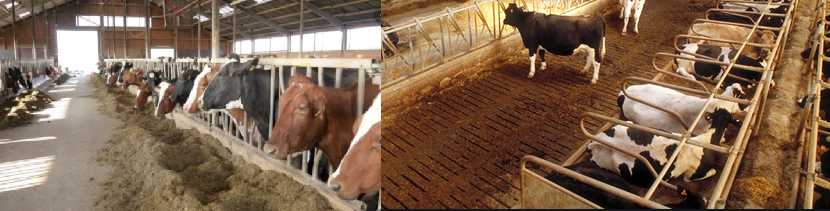
\includegraphics[scale=0.8]{img/estabulado.png}
 \end{center}
 \caption{Sistema de explotación estabulada. Tomada de \cite{googlepics}. \label{estabulpng}}
\end{figure}

El sistema ``estabulado'' (Ver figura \ref{estabulpng}) es una forma de crianza de ganado en la cual los animales pasan la mayor parte del tiempo en establos donde realizan sus actividades diarias. En estos establos se recrea la vida del ganado con la diferencia que el mismo se encuentra protegido bajo techo sin tener exposición directa al sol y a las condiciones medio ambientales. En este sistema se pretende una mayor producción y mejor calidad de la carne en el menor tiempo posible \cite{defestabulacion}.\\

 Por su parte el sistema ``silvopastoril' (ver Figura \ref{silvopng})' es una forma de cultivo agropecuario que involucra la presencia de árboles interactuando con gramíneas y los animales sometidos a un manejo determinado para incrementar la productividad y el beneficio neto de la explotación a mediano y corto plazo \cite{defsilvopas}.

\begin{figure}[H]
 \begin{center}
 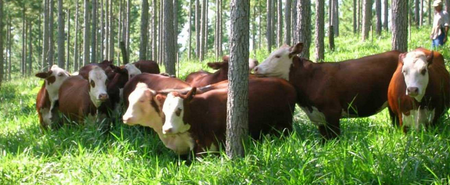
\includegraphics[scale=0.9]{img/silvopastoril.png}
 \end{center}
 \caption{Sistema de explotación silvopastoril. Tomada de \cite{contextoganadero}. \label{silvopng}}
\end{figure}

Finalmente, en el sistema semiestabulado se combinan los 2 sistemas mencionados. En este sistema mixto, los animales ingieren sus raciones de alimento principal en áreas extensas de pastos y forrajes vegetales, mientras que el cuidado y el suministro especializado de vitaminas y proteínas se realiza bajo techo.
%\begin{figure}[H]
% \begin{center}
% \includegraphics[scale=0.6]{img/tiposdosif.png}
% \end{center}
% \caption{Sistema de explotación por estabulación.  \label{estabulpng}}
%\end{figure}
%\begin{figure}[H]
% \begin{center}
% \includegraphics[scale=0.6]{img/tiposdosif.png}
% \end{center}
% \caption{Sistema de explotación silvopastoril. \label{silvopng}}
%\end{figure}
\subsection{Ciclo productivo de la leche}

% 2/10/2022 Cambiar la iamgen por una que tenga que ver con leche y luego descomentar el begin figure 
% \begin{figure}[H]
% \begin{center}
% 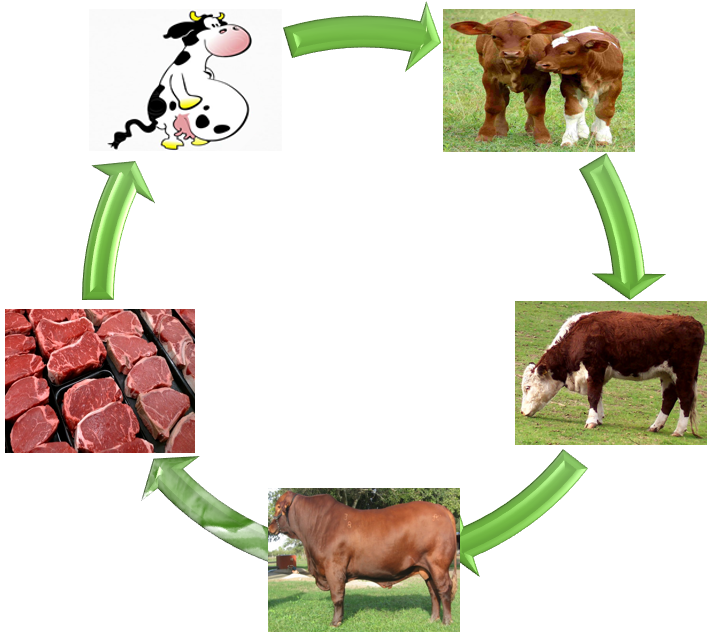
\includegraphics[scale=0.45]{img/ganadcarne.png}
% \end{center}
% \caption{Ciclo productivo en la ganadería de ordeño. \label{ganadcarnepng}}
% \end{figure}

% (Ver Figura \ref{ganadcarnepng}) 
 
El ciclo productivo de la leche de un ganado destinado para tal fin consta de 3 etapas principales que abarcan desde la gestación de la cría y maxima producción de leche, seguido de un periodo de declive y persistencia de producción y finalizando con el periodo de secado en donde se da descanso a la vaca para que se regenere el tejido glandular productor de leche para la siguiente lactancia \cite{mahecha}.\\

Estas etapas son brevemente descritas a continuación:


% \begin{itemize}
    \subsubsection{Etapa de crianza:} Es la etapa de producción temprana en donde el animal (generalmente crías hembras denominadas terneras) son alimentadas y criadas hasta alcanzar 2 años de edad.
	\begin{itemize}
% 		\item En esta etapa se requiere de grandes extensiones de tierra para producir crías
		\item No requiere de estaciones climatológicas específicas y se puede dar en todo el año (Esta característica varía dependiendo de la ubicación geográfica y las exposiciones climatológicas).
		\item Los elementos principales en la dieta de estas criaturas son los nutrientes provenientes del Calostro, la leche materna, forraje y vitaminas.\\
	\end{itemize} 
	\subsubsection{Etapa de gestación y ordeño:} Es la etapa inmediatamente siguiente a la etapa de crianza, en donde la novilla esta desarrollada y en la capacidad de ser inseminada para iniciar su producción de leche.
	\begin{itemize}
% 		\item En esta etapa se estima que el peso del animal puede alcanzar un mínimo de 230[kg] de peso en adelante.
% 		\item Es considerada como la etapa más rentable debido a las  pocas exigencias en materia de calidad alimenticia. 
		\item El objetivo de esta etapa es que la novilla produzca leche mientras que se da la gestación del novillo dentro de ella.
		\item El alimento se basa en pasturas de calidad, provenientes de las extensiones de tierra donde comen las reses y se crían.
		\item El animal gana mayor peso debido a su etapa de crecimiento, por lo que entre mejor sea su alimentación se obtendrán mejores resultados.
		\item Es de vital importancia que el animal se encuentre en la capacidad de  alimentarse \texit{Ad Libitum}, es decir a placer y a voluntad.
		\item En esta etapa, la novilla es denominada primípara, pues se encuentra abarcando el tiempo de gestación de su primera cría.\\
	\end{itemize} 
	\subsubsection{Etapa seca o de secado:} Es la etapa final que abarca los últimos 2 meses de gestación previos al parto en donde se da paso a la regeneración de tejidos glandulares que producen leche y a la curación de las glándulas mamarías para reducir el riesgo de mastitis. En sus características principales se pueden mencionar:
	\begin{itemize}
		\item Aún cuando la novilla primípara esta en capacidad de producir leche, no se debe recurrir al ordeño hasta que no se realice el parto.
	\end{itemize}
% \end{itemize} 

\subsubsection{Razas}

Debido a la gran variedad de especies, condiciones ambientales, y al proceso evolutivo del ganado, históricamente se ha podido clasificar y seleccionar las razas más representativas para este tipo de explotación ganadera. Más precisamente se puede hacer mención de las siguientes:
\begin{multicols}{2}
    \begin{center}
        \begin{itemize}
        \item Simmental
        \item Holstein
        \item Jersey
        \item Normando
        \end{itemize}
    \end{center}
\end{multicols}

Éstas son seleccionadas principalmente por la contextura voluminosa pero factores como la calidad de la leche pueden sobrepasar los criterios cuantitativos. A continuación se muestran algunos ejemplares de estas razas:

\begin{figure}[H]
 \begin{center}
 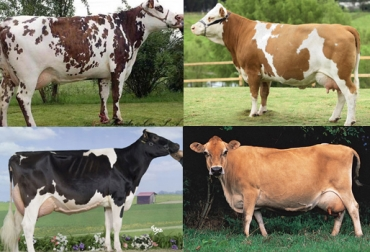
\includegraphics[scale=1]{img/razaslecheras.png}
% \end{center}
 \caption{En la primer fila de izquierda a derecha se observan ejemplares de las razas Normando, Simmental; seguido de las razas Holstein y Jersey en la fila inferior. Tomada de \cite{contextoganadero} \label{cuadrorazaspng}}
  \end{center}
\end{figure}

\subsection{Ciclo productivo de la carne}

\begin{figure}[H]
\begin{center}
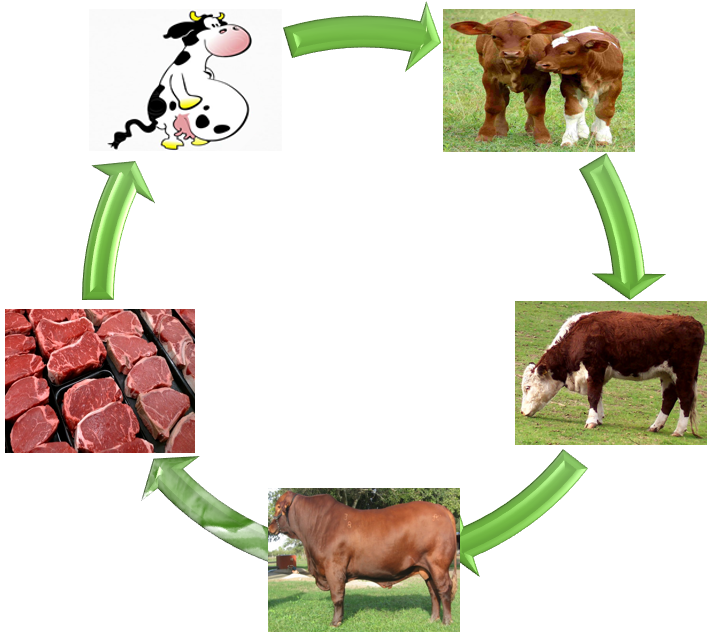
\includegraphics[scale=0.55]{img/ganadcarne.png}
\end{center}
\caption{Ciclo productivo en la ganadería de la carne.  Tomada de \cite{contextoganadero}. \label{ganadcarnepng}}
\end{figure}

 
El ciclo productivo de la carne (Ver Figura \ref{ganadcarnepng})  de un ganado destinado para tal fin consta de 3 etapas principales que abarcan desde el nacimiento de la cría, su desarrollo y crecimiento y finalizando con su comercialización en el momento en que alcanza las condiciones apropiadas para ser transformado en carne para consumo humano \cite{mahecha}. Estas etapas son brevemente descritas a continuación:


%y finalizando en el momento en que alacanza las condiciones apropiadas para ser transformado en carne para consumo humano \cite{mahecha}. Estas etapas son brevemente descritas a continuación:

\begin{itemize}
	\item \textbf{Ganadería de Cría:} Es la etapa de producción temprana en donde el animal (generalmente crías macho llamadas bovinos) es alimentado y criado desde su nacimiento hasta los primeros seis (6) meses de edad. 
	\begin{itemize}
		\item En esta etapa se requiere de grandes extensiones de tierra para producir crías
		\item No requiere de estaciones climatológicas específicas y se puede dar en todo el año.
		\item Los elementos principales en la dieta de estas criaturas son los nutrientes provenientes del Calostro y la leche materna.\\
	\end{itemize} 
	\item \textbf{Ganadería de Levante:} Es la etapa inmediatamente siguiente a la etapa de crianza, en donde el bovino se desarrollará entre los siete (7) y diez y ocho (18) meses de edad.
	\begin{itemize}
		\item En esta etapa se estima que el peso del animal puede alcanzar un mínimo de 230[kg] de peso en adelante.
		\item Es considerada como la etapa más rentable debido a las  pocas exigencias en materia de calidad alimenticia. 
		\item El objetivo de esta etapa es que el sujeto en cuestión alcance el peso deseado en el menor tiempo posible con el menor esfuerzo posible
		\item El alimento se basa en pasturas de calidad, provenientes de las extensiones de tierra donde comen las reses y se crían.
		\item El animal gana mayor peso debido a su etapa de crecimiento, por lo que entre mejor sea su alimentación se obtendrán mejores resultados.
		\item Es de vital importancia que el animal se encuentre en la capacidad de  alimentarse \texit{Ad Libitum}, es decir a placer y a voluntad.\\
	\end{itemize} 
	\item \textbf{Ganadería de engorde o Ceba:} Es la etapa final que abarca desde los 19 meses de edad hasta los 24 o 36 meses, dependiendo de su crecimiento  y otros factores como el interés del productor, la demanda del mercado, entre otras. En sus características principales se pueden mencionar:
	\begin{itemize}
		\item El límite se define por los intereses del productor, la demanda del mercado y en general por el peso ideal del animal que es aproximadamente mayor o igual a los 450[kg].
		\item Para la alimentación se requieren de buenas, grandes y controladas cantidades con el fin de mejorar la carne. Para esto se utilizan dietas que requieren pasturas y concentrados dietarios.
		\item Se debe monitorear la alimentación tomando registro en la ganancia de gramaje diaria de cada uno de los animales.
	\end{itemize}
\end{itemize} 

\subsubsection{Razas} Debido a la gran variedad de especies, condiciones ambientales, y al proceso evolutivo del ganado, históricamente se ha podido clasificar y seleccionar las razas más representativas para este tipo de explotación ganadera. Más precisamente se puede hacer mención de las siguientes:
\begin{multicols}{2}
\begin{center}
\begin{itemize}
\item Beefmaster
\item Charolais
\item Simmental
\item Angus
\item Brangus
\item Santa Gertrudis
\item Hereford
\item Limousin
\item Cebú
\item Belgina Blue
\end{itemize}
\end{center}
\end{multicols}

Éstas son seleccionadas principalmente por la contextura voluminosa pero factores como la calidad de la carne pueden sobrepasar los criterios cuantitativos. A continuación se muestran algunas de las razas más usadas para este propósito:

\begin{figure}[H]
 \begin{center}
 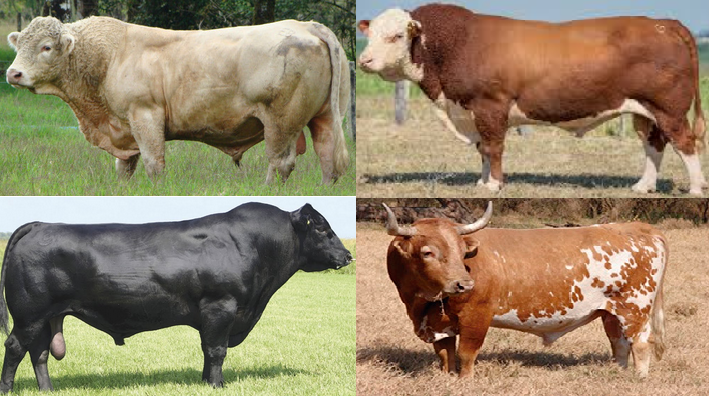
\includegraphics[scale=0.8]{img/cuadrorazas.png}
% \end{center}
 \caption{En la primer fila de izquierda a derecha se observan ejemplares de las razas Charolais, Hereford; seguido de las razas Angus y Criolla en la fila inferior.  Tomada de \cite{contextoganadero}. \label{cuadrorazaspng}}
  \end{center}
\end{figure}


\subsection{Alimentación y Componentes básicos de la dieta}
%\section{Marco de referencia}
% \subsubsection{Alimentación}
La alimentación de un cultivo de ganado requiere de una dieta o ración con diferentes componentes básicos o nutrientes que deben ser suministrados día a día de forma balanceada para lograr un crecimiento óptimo y que los animales puedan expresar su potencial genético \cite{recomendaciones}.\\

Los componentes principales que conforman la dieta alimenticia  del ganado son:
% 	\begin{itemize}
	

\subsubsection{Agua}
    Componente principal de la alimentación. Esta debe ser suministrada en cantidad y calidad para ser aprovechada por cada animal llegando a ocupar más del 50\% de la masa corporal de un ejemplar adulto y hasta un 90 \% de un recién nacido.
    	
	\begin{figure}[H]
	 \begin{center}
	 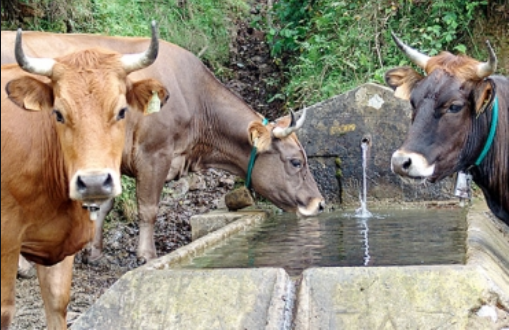
\includegraphics[scale=0.8]{img/agua.png}
	 \end{center}
	 \caption{Hidratación del ganado. Tomada de \cite{contextoganadero}.	\label{energeticospng}}
	\end{figure}
    	
\subsection{Energía}
Este componente se suministra mediante azúcares, almidones, celulosa, entre otros, los cuales aportan grandes cantidades de energía mas no de proteína, razón por la cual se deben suministrar de forma complementaria.
	\begin{figure}[H]
	 \begin{center}
	 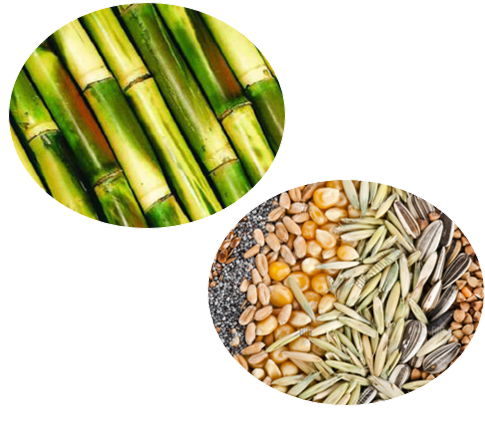
\includegraphics[scale=0.7]{img/melazacana.png}
	 \end{center}
	 \caption{Suplementos energéticos. 	\label{energeticospng}}
	\end{figure}
    
\subsection{Proteínas}
Estos nutrientes son fundamentales especialmente durante los periodos de sequía, por consiguiente, se optan por fuentes altas en proteína como leguminosas forrajeras, el Maní, Leucaena y el más común, los pastos de forraje verde. 
	\begin{figure}[H]
	 \begin{center}
	 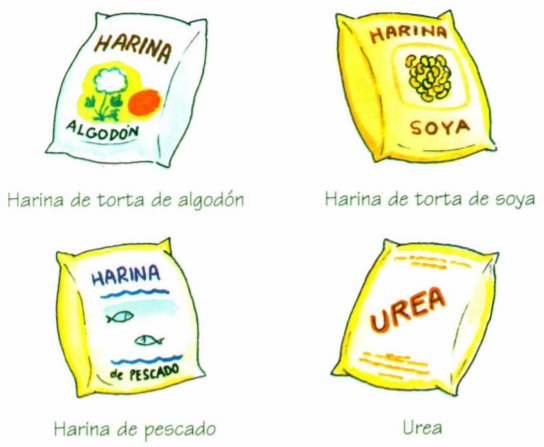
\includegraphics[scale=0.8]{img/proteina.png}
	 \end{center}
	 \caption{Suplementos proteínicos. Tomada de \cite{librito1}. \label{proteinaspng}}
	\end{figure}

\subsection{Minerales}
Son indispensables en la ganancia de peso de los novillos durante la etapa de Cría y Levante. Este complemento alimenticio debe estar siempre a la disposición para que el ganado pueda abastecer sus necesidades. Estos minerales se suelen proporcionar mediante mezclas de macrominerales y microminerales que se ofrecen de libre consumo al ganado.

\subsection{Vitaminas}
Suministradas en cantidades pequeñas aplicadas comúnmente en animales cuya alimentación se basa en forrajes secos,  o en animales enfermos convalecientes, desnutridos o durante épocas de sequía prolongada.
	\begin{figure}[H]
	 \begin{center}
	 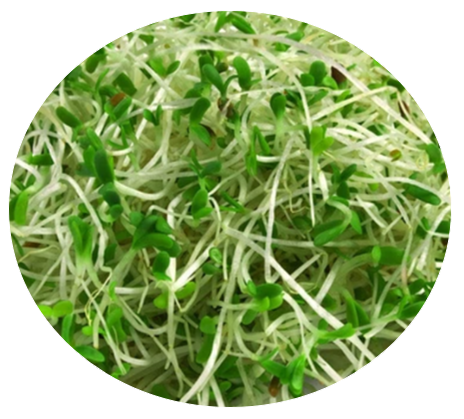
\includegraphics[scale=0.6]{img/leguminosas.png}
	 \end{center}
	 \caption{Forraje y leguminosas. Tomada de \cite{librito1}. \label{vitaminaspng}}
	\end{figure}

\subsection{Balance de raciones y dietas especializadas}
% \subsubsection{Balance de raciones y dietas especializadas}
    Estas dietas son suministradas por personal técnico calificado que prepara un dieta acorde a la cantidad de nutrientes de cada animal de forma particular e independiente, considerando su peso actual, su velocidad de crecimiento y estado fisiológico.

\subsection{Desperdicios}

\section{Leyes y Normatividad}  \label{leyes}
Requerida para que el avance ganadero se realice de manera coordinada o estandarizada basada en las buenas prácticas ganaderas en pro de mejorar la productividad y ayudarla a alcanzar niveles de ganadería bovina del mundo \cite{invima}, \cite{leylacteos}, \cite{minsaludleche}. 
\begin{itemize}
	\item \textbf{Resolución 2310 de 1986:} Reglamentación parcial en el titulo V de la ley 09 de 1979 que se refiere al procesamiento, composición, requisitos, transporte, y comercialización de los Derivados Lácteos.
	\item \textbf{Resolución 11961 de 1989:} Reglamentación parcial a la resolución 2310 de 1986 que se refiere a lo relacionado con las clases de leche fermentada.
	\item \textbf{Decreto 0616 de 2006:} Reglamento técnico sobre los requisitos que debe cumplir la leche para el consumo humano que se obtenga, procese, envase, transporte, comercialice, expenda, importe o exporte en el país.
	\item \textbf{Resolución 0012 de 2007:} Por la cual se establece el sistema de pago de la leche cruda al productor, diseñado por la Unidad de Seguimiento de Precios.
	\item \textbf{Decreto 1500 de 2007:} Reglamento técnico a través del cual se crea el Sistema Oficial de Inspección, Vigilancia y Control de la Carne y otros productos comestibles y derivados cárnicos destinados para el consumo humano.
	\item \textbf{Decreto 072 de 2007:} Por el cual se establece el manual de buenas prácticas de manejo para la producción de ganado bovino.
	\item \textbf{Decreto 2905 de 2007:} Por el cual se establece el reglamento técnico sobre los requisitos sanitarios y de inocuidad de la carne y productos cárnicos comestibles de las especies bovina y bufalina destinados para el consumo humano.
	\item \textbf{Decreto 18119 de 2007:} Por el cual se reglamenta los requisitos del plan gradual de cumplimiento para  las plantas de beneficio y desposte de bovino y bufalinos.
	\item \textbf{Decreto 2278 de 1982:} Reglamentación parcial en el titulo V de la ley 09 de 1979 que se refiere al sacrificio de animales de abasto público o para consumo humano y el procesamiento, transporte y comercialización de su carne.

\end{itemize}

% \section{Conceptos adicionales}
% \item \textbf{Jáquima:} Es un freno, cabestro o cabezada usado en la ganadería principalmente equina, para identificar, amansar o manipular al animal \cite{jaquima}.

% %%%%%Productos y resultados que se entregarán cuando finalice el proyecto (1/2 página). 


%%%%%%%%%%%%%%%%%%%%%%
% DESCRIPCION DEL PROBLEMA
%%%%%%%%%%%%%%%%%%%%%%
\chapter{Descripci\'on del Problema}

%%%%%%%%%%%%%%%%%%%%%%
% DESCRIPCION DEL PROBLEMA
%%%%%%%%%%%%%%%%%%%%%%

\section{Planteamiento del Problema} \label{plant}
%ESTO SE BORRA-> Explicar el CONTEXTO, s\'intomas y causas del problema a resolver. (1.5 p\'aginas).EXPLICAR QUE VOY A HACER \\ \\

El sector ganadero abarca diferentes especies de ganado tales como, los bovinos, los ovinos, los porcinos, entre otros. En Colombia se tiene una alta presencia de producción de estos tipos especialmente en el ganado bovino y ovino. De igual forma, estos tipos de ganado tienen diferentes modalidades, entre las cuales se pueden mencionar el ganado para crianza, para producción de leches y sus derivados y ganadería de la carne. En Colombia y el mundo se presentan constantes inversiones en materia tecnológica para mejorar la forma en cómo el ganado es productivo y puede participar de forma competitiva en un mercado de consumo de calidad.\\

Debido a que el ciclo productivo de la carne consta de diferentes etapas con diferentes requerimientos, necesidades y cantidad de áreas verdes, se considera aportar el diseño de un sistema que pueda simplificar  tareas de obtención de datos y gastos por mano de obra en cultivos de reses destinados al engorde, los cuales pueden desempeñarse en espacios cerrados como establos, dando paso al monitoreo por condiciones de estabulación, en donde se garantiza el suministro de forraje verde, minerales, vitaminas y dietas específicas para el ganado y adaptándose a espacios cercanos a la casa matriz de administración de los productores \cite{contextoganadero}.
En el Cauca, aunque se cuente con bastas hectáreas de diferentes fertilidades y condiciones térmicas apropiadas para el cultivo y desarrollo de la ganadería, se presentan muchas falencias en materia tecnológica y económica, en donde los movimientos migratorios de campesinos desplazados y los efectos colaterales del conflicto armado que se ha presentado en el país, son las principales causas de estas falencias. Sin embargo, el emprendimiento de los pequeños y medianos productores da paso a nuevas oportunidades de intervención por parte de la Ingeniería electrónica y el manejo aplicativo de nuevas tecnologías que permitan tener un contacto más cercano con la población campesina. \\

El manejo de software sofisticado y maquinaria industrial puede presuponer brechas para con los usuarios campesinos por la falta de capacitación técnica o por la complejidad de uso de los programas para el manejo de datos. Sin embargo, el desarrollo de nuevas tecnologías ha dado paso a una era digital con la que se espera lograr avances significativos. Como se menciona en \cite{minagricultura}, \cite{ashby} y \cite{fao} la inclusión de las ciencias y la formación de entidades de apoyo al sector agrario pueden aportar significativamente al desempeño de los  cultivos ganaderos. 
Como medio para facilitar al usuario la inclusión de software y herramientas tecnológicas más amigables se plantea el manejo de una HMI para que por medio de ésta, el usuario ganadero pueda añadir o eliminar uno o mas reses, establecer los valores dietarios, asignar los RFID a nuevos novillos, visualizar (en caso que se presente) avisos o alarmas y encender o apagar el sistema.\\

Lo anterior se diseña, y se plantea acorde con el manual de Buenas Prácticas de Ganadería  (BPG) y con las legislaciones pertinentes al manejo de alimentos para el consumo humano establecidas por la ley colombiana mencionados en la sección \ref{leyes}.

%%%%%%%%% CREOQ UE ESTE PARRAFO SE PUEDE BORRAR:
%%se puede reprogramar y reconfigurar la cantidad de  micro controladores como Arduino o Rasperry Pi \cite{arduinodef}. Estos dispositivos son fácilmente re-programables y pueden adaptarse no solo a las necesidades de pequeños productores ganaderos sino también al uso por parte de grandes cultivadores del ganado de la carne.\\






%%%%%%%%%%%%%%%%%%%%%%%%%%%
%%%%  TRABAJOS FUTUROS
%%%%%%%%%%%%%%%%%%%%%%%%
%%%%
%%%%Para trabajos futuros y de mayores dificultades geograficas se considera la posibilidad de acceder a los datos de manera remota mediante las redes de Internet y datos, y estableciendo un sistema automático de suministro y supervisión alimenticio; con esto se espera reducir gastos por transporte, personal de seguimiento y tiempo  y claridad en el registro de datos dando así, paso para que estos tiempos y recursos puedan ser redistribuidos en otras o nuevas tareas del productor ganadero.









\subsection{Formulaci\'on}
%Pregunta fundamental que se busca responder con el proyecto en esta formulación.

%%?`C\'omo detectar la presencia de deformaci\'on de pavimentos en un tramo vial para posteriormente realizar una plataforma basada en la informaci\'on recolectada colectivamente por los usuarios del sistema? %en esta formulación 

?`Cómo monitorear de manera automática la evolución alimenticia de reses en proceso de ceba bajo condiciones de estabulación para productores ganaderos de carne? 

%?`Cómo monitorear la evolución alimenticia de reses en proceso de ceba mediante un sistema automático de bajo costo para productores ganaderos de carne? 

\subsection{Sistematizaci\'on}
%Subpreguntas que ayudan a definir claramente el problema de investigaci\'on (1 p\'agina con la formulaci\'on) 			
El problema se sistematiza de la siguiente manera:
\begin{itemize}
	\item ?`Qué tipo de herramientas tecnológicas se utilizar\'ian para realizar el monitoreo alimenticio de las reses?
	\item ?`C\'omo identificar cada cabeza de ganado por separado y evitar confusiones en grandes poblaciones de ganado?
	\item ?`C\'omo saber los tiempos del día en los que se debe suministrar el alimento?
%	\item ?`C\'omo saber la cantidad de alimento que será suministrado en un día y verificar que aún se cuente con alimento suficiente para ser suministrado al ganado?
	\item ?`C\'omo verificar que aún se cuente con alimento suficiente para ser suministrado al ganado?
	\item ?`C\'omo saber la porción de alimento apropiada para cada animal de manera particular?
	\item ?`C\'omo suministrar el alimento racionado?
	\item ?`C\'omo verificar que no se otorgará de manera equívoca las porciones de alimento a animales erróneos?
	\item ?`C\'omo verificar que una res en particular ha ingerido correctamente su porción de alimento?
	\item ?`C\'omo verificar que una res determinada presenta (o no) un crecimiento de peso acorde a los intereses del productor?
	\item ?`C\'omo verificar que una res en específico ha alcanzado su peso máximo o ideal de acuerdo con los intereses del productor?
	\item ?`C\'omo notificar cuando no haya suficiente alimento para suministrarlo a el ganado?
	\item ?`C\'omo registrar los datos sensados en una base de datos en la nube?
	\item ?`C\'omo realizar el registro de forma automática?
	\item ?`C\'omo mostrar al usuario los datos registrados en la base de datos?
	\item ?`C\'omo representar los datos almacenados en la base de datos?
	\item ?`C\'omo verificar que los resultados obtenidos son acordes al diseño planteado?
\end{itemize}

\section{Objetivos}
\subsection{Objetivo General}

%\textbf{\textit{aksjhfkajhsgfkajshfkasj}}

Diseñar un sistema de monitoreo alimenticio con herramientas de bajo costo para ganado estabulado en proceso de ceba.


\subsection{Objetivos Espec\'ificos}

\begin{itemize}
	\item Investigar, clasificar y seleccionar los dispositivos y herramientas que serán usadas para el sensado de la deformación.
	\item Asignar números, nombres  o características de identificación para referenciar a cada res.
	\item Utilizar dispositivos de tiempo para poner en funcionamiento el alimentador a las horas deseadas por el productor.
	\item Comprobar la existencia de cantidad suficiente de alimento almacenado.
	\item Suministrar la porción de alimento respectiva a cada bovino mediante la cantidad especificada por su referencia de identificación.
	\item Entregar la ración de alimento mediante un actuador de dosificación.
	\item Identificar a la res mediante su referencia de identificación y corroborar si ya se le ha suministrado (o no) su respectiva porción de alimento en una franja horaria determinada.
	\item Corroborar que la res ha ingerido su porción de alimento
	\item Monitorear el crecimiento de peso de cada res y compararlo con el crecimiento ideal o deseado.
	\item Conocer el peso de cada cabeza de ganado diariamente.
	\item Notificar al personal encargado la insuficiencia de alimento almacenado.
	\item Registrar la información sensada en una unidad de almacenamiento en la nube.
	\item Realizar el registro de datos de forma automática.
	\item Permitir al usuario acceder a los datos almacenados.
	\item Representar los datos almacenados de manera gráfica.
	\item Realizar un plan de pruebas.
\end{itemize}


\textbf{\section{Justificaci\'on}}
%\textbf{\textit{Justificaci\'on del proyecto (metodol\'ogica, te\'orica, pr\'actica) (1 p\'agina)}}

%%%%%%%%%%        ALIMENTO DE RESES DE CEBA DE RESES ESTABULADAS       %%%%%%%%%%%%%%%%%%%%%%%%%%%%%%%%%%%%%%

La ganadería de la carne supone un ambiente apropiado para que los animales en cuestión puedan sacar provecho de sus  cualidades genéticas y puedan producir los mejores productos en cuestión de calidad. Para ello, el cultivo de la carne debe ser debida y minuciosamente realizado lo que supone un constante trabajo de inspección tanto de la alimentación del ganado así como también del registro apropiado de los datos de seguimiento determinados por el ganadero y los intereses del mercado.
Sin embargo, las fincas y los terrenos destinados para estabular el ganado suelen encontrarse en recintos separados lo que implica a los productores tener un constante transporte de bienes y recursos tanto físicos como personales, lo que conlleva a gastos de recursos en transporte y contratación de personal. Además se debe llevar un registro de las especificaciones alimenticias y dietarías de cada res con lo que se presuponen grandes tareas de registro de actividades y datos primarios sobre el proceso evolutivo de la alimentación del ganado. No obstante, estas tareas de registro son realizadas de manera general abarcando el comportamiento general del ganado alimentado y en ocasiones se presentan casos en donde se distribuye de manera desorganizada conjunta del alimento dietario, ocasionando que algunas reses puedan abastecerse de dietas más desproporcionadas que otras lo que conlleva de comportamientos en peso irregulares o poco deseados para los intereses de los productores.

En este trabajo se propone un alimentador automático de bajo costo para reses en proceso de engorde o ceba que permita, mediante sensores de peso, suministrar una cantidad de alimento de manera automática para cada res, en horarios del día preestablecidos por el productor ganadero y cuya ración será respectiva a la dieta de cada animal basada en los intereses del propietario. Las reses estarían identificadas por un número ID unido directa o indirectamente a sus cuerpos con lo cual se supervisa cada bovino por separado generando un historial alimenticio en la nube para cada individuo. Este historial permitiría organizar de manera sistemática el proceso evolutivo de la alimentación de una res específica sin prestaciones a errores humanos por registro indebido o erróneo.
Por medio de este alimentador se generaría un historial alimenticio de cada bovino que permitiría registrar la cantidad de porciones suministradas periódicamente, además de verificar, con sensores de presencia o detección,  si éste ha ingerido su alimento o no con lo cual se podrá identificar aquellas cabezas de ganado que estarían presentando desordenes alimenticios que vayan en contra de los intereses del productor. Esto aportaría significativamente a un distribución más sistemática  y eficiente del alimento del ganado.\\

Entre los datos fijos de cada historial se tendría registro de su Nombre, RFID, Sexo, Raza, Peso y Edad inicial, Peso y Edad final; y como datos de monitoreo se tendría registro diario peso, edad, peso máximo alcanzado, si ha alcanzado o no un peso ideal y su evolución del peso para verificar si está obteniendo un crecimiento positivo, o en caso contrario, proceder con la toma de decisiones respecto al sujeto en cuestión tales como su posible venta, tratamiento, o venta temprana, entre otros.

Al estar identificados con un número ID propio e independiente, mediante un sensor RFID, se ayuda a que el alimento se suministre al individuo correcto y que no se presentan casos en los que se suministren porciones repetidas en una misma franja horaria. Una vez el animal se encuentre en la zona de alimentación, estos serán pesados con el objetivo de hacer seguimiento del crecimiento de peso y verificar que esté cumpliendo con la tasa de crecimiento fijada por el productor y en caso de alcanzar un peso máximo preestablecido o presentar disminución de peso hacer la respectiva notificación y observación en la nube para la toma de decisiones futuras.\\

Por último el sistema verifica la cantidad neta de alimento suministrado y dará aviso preventivo, mediante un recordatorio o una alarma al personal encargado notificando si el alimento está próximo a acabarse.
Es importante resaltar que este sistema se realiza con herramientas y sensores de bajo costo de Arduino.\\





\section{Delimitaciones y Alcances} \label{limites}
\begin{itemize}
	\item La programación se realiza en Arduino como herramienta de procesamiento de los datos en crudo sensados.
	\item Se utilizarán módulos y sensores de bajo costo en comparación a sensores de nivel industrial.
	\item Los módulos actuadores y de sensado además de los parámetros de entrada usados en el prototipo, representarán (a escala) los valores y comportamientos de parámetros y sensores usados en trabajos de campo a nivel comercial. %(VER COMO ESCRIBIRLO MEJOR)
%	\item Se hará una búsqueda y clasificación de dispositivos para el sensado de las variables estables y evolutivas que serán monitoreadas. (ESTO PARECE MAS QUE TODO UNA ACTIVIDAD) -> LISTO EL POLLO
	\item Se seleccionarán los dispositivos más acordes a las necesidades y recursos limitados de y para el desarrollo del proyecto.
	\item El (los) algoritmo(s) será(n) probado(s) en la construcción del prototipo maqueta a escala mas no en una implementación final en infraestructura ganadera ya establecida.
	\item El diseño del sistema final entregado da la posibilidad de implementar un sistema con hasta 4 dosificadores por 1 solo contenedor o almacenador de alimento.
	\item El prototipo final a entregar constaría de la funcionalidad del sistema para 1 solo punto de dosificación del alimento.
	\item La notificaci\'on se registra en una base de datos. En caso de ser física, en un archivo de texto con modalidad .csv; en caso de ser en la nube, en Google Drive. El registro de la notificación hace parte del prototipo realizado.
	\item El envío de los datos a la nube se realiza mediante módulos Wifi de Arduino Esp8266.
	\item Los registros en la base de datos se caracterizar\'ian por los datos procesados obtenidos en el sensado.
	\item El sistema diseñado es prototipable o implementable para territorios con acceso a Internet.

%	\item 	Se dise\~na una aplicaci\'on m\'ovil  con la que se podrá verificar los registros de deformaciones.
\end{itemize}

%Enumere las delimitaciones (restricciones) en la soluci\'on que va a proponer.  (1/2 p\'agina). 
\subsection{Entregables}
Se establece diseñar un prototipo que constaría de:

\begin{itemize}
	\item Diseño de un sistema automático de monitoreo alimenticio de reses estabuladas en proceso de ceba.  
	\item Diseño de Prototipo funcional (a escala) del sistema diseñado con un único punto de dosificación.
	\item Construcción física (a escala) del prototipo diseñado con un solo dosificador funcional.
	\item Plan de pruebas.
	\item Documentación descriptiva, explicativa y argumentativa que evidencie el proceso de desarrollo del proyecto.
\end{itemize}
%Productos y resultados que se entregar\'an cuando finalice el proyecto (1/2 p\'agina). 




%%%%%%%%%%%%%%%%%%%%%%
% DESARROLLO DEL PROYECTO
%%%%%%%%%%%%%%%%%%%%%%

\chapter{Desarrollo del Proyecto} 
%%%%%%%%%%%%%%%%%%%%
% DESARROLLO DEL PROYECTO
%%%%%%%%%%%%%%%%%%%%

\section{Marco de Referencia}
\subsection{\'Areas Tem\'aticas}
\begin{itemize}
	\item Algoritmos computacionales.
	\item Almacenamiento en la nube.
	\item Bases de datos digitales.
	\item Ciencias agropecuarias. %agricolas? y pecuarias?
	\item Ganadería de carne.
	\item Ingeniería electrónica.
	\item Monitoreo digital.
	\item Sistemas RFID.
\end{itemize}

\subsection{Marco Te\'orico}

%Este proyecto consiste en el desarrollo de un sistema automático de bajo costo para el monitoreo de la alimentación de ganado involucrado en el ciclo productivo en la denominada "Ganadería de la Carne", es decir, reses que se encuentren en proceso de engorde o Ceba.
%El sistema podrá, mediante una variedad de sensores (peso, presencia y/o detección, tiempo real, RFID, comunicación vía Wifi), monitorear la alimentación respectiva de cada cabeza de ganado de forma particular e independiente de las demás mediante la toma y registro de datos en bases de datos en la nube. Esto se plantea mediante una propuesta electrónica basada en nuevas tecnologías y manejo de algoritmos computacionales.

%En este documento se propone un alimentador automático de bajo costo para reses en proceso de engorde o ceba que permita, mediante sensores de peso, suministrar una cantidad de alimento de manera automática para cada res, en horarios del día preestablecidos por el productor ganadero y cuya ración será respectiva al la dieta de cada animal basada en los intereses del propietario. Las reses estarían identificadas por un número ID colgando de sus cuerpos con lo cual se monitorea cada bovino por separado generando un historial alimenticio en la nube para cada individuo.
%Por medio de este alimentador se generaría un historial alimenticio de cada bovino que permitiría registrar la cantidad de porciones suministradas periódicamente, además de verificar, con sensores de presencia o detección,  si éste ha ingerido su alimento o no con lo cual se podrá identificar aquellas cabezas de ganado que estarían presentando desordenes alimenticios que vayan en contra de los intereses del productor.\\
%
%Entre los datos fijos de cada historial se tendría registro de su Nombre, RFID, Sexo, Raza, Peso y Edad inicial, Peso y Edad final; y como datos de monitoreo se tendría registro diario peso, edad, peso máximo alcanzado, si ha alcanzado o no un peso ideal y su evolución del peso para verificar si esta obteniendo un crecimiento positivo, o en caso contrario, proceder con la toma de decisiones respecto al sujeto en cuestión tales como su posible venta, tratamiento, o venta temprana, entre otros.
%
%Al estar identificados con un número ID propio e independiente, se ayuda se garantiza, mediante un sensor RFID, que el alimento se suministra al individuo correcto y que no se presentan casos en los que se suministren porciones repetidas en una misma franja horaria. Una vez el animal se encuentre en la zona de alimentación, estos serán pesados con el objetivo de hacer seguimiento del crecimiento de peso y verificar que esté cumpliendo con la rata de crecimiento fijada por el productor y en caso de alcanzar un peso máximo preestablecido o presentar disminución de peso hacer la respectiva notificación y observación en la nube para la toma de decisiones futuras.\\
%
%Por último el sistema verifica la cantidad neta de alimento suministrado y dará aviso preventivo, mediante un recordatorio o una alarma al personal encargado notificando si el alimento está próximo a acabarse.
%Es importante resaltar que este sistema se realiza con herramientas y sensores de bajo costo de Arduino.

%algoritmos que permitan obtener grandes cantidades de informaci\'on registrada en una base de datos para que esta información sirva como base para determinar tramos viales con mayor o menor deterioro vial. Esto se plantea mediante una propuesta electr\'onica basada en nuevas tecnolo\'ias y algoritmos computacionales.


\subsubsection{Alimentación}
La alimentación de un cultivo de ganado requiere de una dieta o ración con diferentes componentes básicos o nutrientes que deben ser suministrados día a día de forma balanceada para lograr un crecimiento óptimo y que los animales puedan expresar su potencial genético \cite{recomendaciones}. Los componentes principales que conforman la dieta alimenticia del ganado son:
	\begin{itemize}
	\item \textbf{Componentes básicos de la dieta} % Ponerle negrilla
		\begin{itemize}
		\item Agua: Componente principal de la alimentación. Esta debe ser suministrada en cantidad y calidad para ser aprovechada por cada animal llegando a ocupar mas del 50\% de la masa corporal de un ejemplar adulto y hasta un 90 \% de un recién nacido.
		\item Energía:  Este componente se suministra mediante azúcares, almidones, celulosa, entre otros, los cuales aportan grandes cantidades de energía mas no de proteína, razón por la cual se deben suministrar de forma complementaria.
		\item Proteínas: Estos nutrientes son fundamentales especialmente durantes los periodos de sequía para lo cual se optan por fuentes altas en proteína como leguminosas forrajeras como el Maní, Leucaena y el más común, los pastos de forraje verde. 
		\item Minerales: Son indispensables en la ganancia de peso de los novillos durante la etapa de Cría y Levante. Este complemento alimenticio debe estar siempre a la disposición para que el ganado pueda abastecer sus necesidades. Estos minerales se suelen proporcionar mediante mezclas de macrominerales y microminerales que se ofrecen de libre consumo al ganado.
		\item Vitaminas: Suministradas en cantidades pequeñas aplicadas comúnmente en animales cuya alimentación se basa en forrajes secos,  o en animales enfermos convalecientes, desnutridos o durante epocas de sequía prolongada.
		\end{itemize}
	\item \textbf{Balance de raciones y dietas especializadas} %Ponerle negrilla
Estas dietas son suministradas por personal técnico calificado que prepara un dieta acorde a la cantidad de nutrientes de cada animal de forma particular e independiente, considerando su peso actual, su velocidad de crecimiento y estado fisiológico.
	\end{itemize}
	
	
\subsubsection{Almacenamiento}
El alimento almacenado cae por gravedad al mecanismo de dosificación y este debe ser adaptado a su tamaño, densidad y peso \cite{pinturan}. Aparte del mecanismo, se debe tener en cuenta el material de contrucción, entre los materiales de fabricación mas comunes se encuentran el Poliestireno, Vidrio  y Céramica, Acero Inoxidable, Plástico,  entre otros. Estos deben garantizar resistencia y que cumpla con los requerimientos generales de almacenamiento de alimentos \cite{casti}:
\begin{itemize}
	\item El material de fabricación no debe modificar la composición, color, sabor, ni olor del producto contenido y no puede ceder componentes al medio interno ni externo que constituyan un riesgo para la salud.
	\item Fabricación con polímeros y aditivos que están incluidos en las listas positivas de las regulaciones alimentarias.
	\item Cumplir con los requisitos específicos de migración total en casos de compuestos químicos y componentes en el material plástico.
\end{itemize}


\subsubsection{Mecanismos de Dosificación}
El suministro de los alimentos del ganado cultivado se realiza mediante dispositivos electrónicos, mecánicos, electromecánicos y manuales. Estos dispositivos regulan el despacho del alimento en las diferentes etapas del cultivo de carne. A modo general, están compuestos por servomotores, motores eléctricos, cilindros neumáticos y/o reguladores electrónicos y mecánicos \cite{pinturan}. 
También pueden ser clasificados acorde a la naturaleza de la sustancia a manipular. Más propiamente dentro de la categoría de dosificadores volumetricos de sólidos secos, existen una gran variedad de mecanismos de dosificación  \cite{torres}, como algunos mencionados a continuación:

	\begin{itemize}
	
		\item \textbf{Dosificadores de Tornillo} % PONER NEGRILLA
		
		En estos dosificadores (Ver figura \ref{torni}) se tiene un Tornillo sin fin que actua como dosificador, éste se suele encontrar en la parte inferior de la tolva de alimentación y libera un volumen determinado de sustancia en cada vuelta; su velocidad y precisión de dosificación dependen de la velocidad de giro con la que se esté manipulando \cite{torres}. Este sistema de dosificación es el más utilizado debido a su implementación simple y porque se adapta a la naturaleza de la mayoría de las sustancias dosificadas.
		\begin{figure}[H]
			\begin{center}
				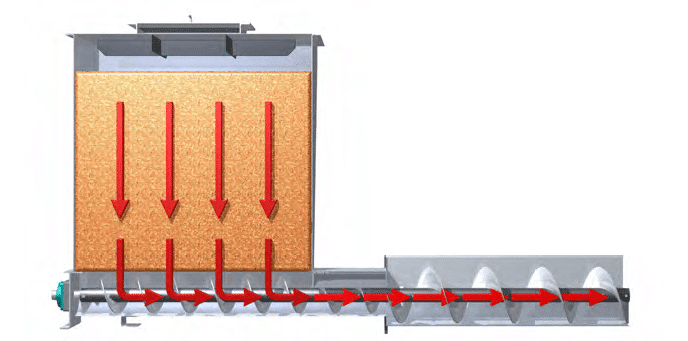
\includegraphics[scale=0.7]{img/tornillo.png}
			\end{center}
			\caption{Mecanismo de Tornillo sin fin. Tomada de \cite{DEM} \label{torni}}
		\end{figure} % Ponerle negrilla
		
		\item \textbf{Dosificadores de Compuerta Rotativa} % PONER NEGRILLA
		
		En este caso se tiene una compuerta rotativa como elemento principal de dosificación, permite una construcción simple y robusta, aunque presenta menor precisión que el mecanismo de tornillo sin fin. Una representación de este tipo de mecanismo se puede ver en la Figura \ref{rotala}.
		\begin{figure}[H]
			\begin{center}
				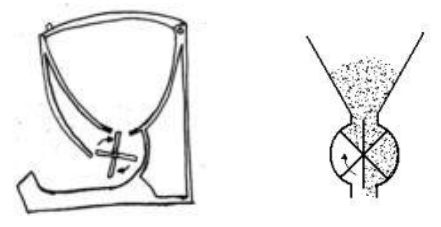
\includegraphics[scale=0.9]{img/rotar.png}
			\end{center}
			\caption{Mecanismo de Compuerta Rotativa. \label{rotala}}
		\end{figure} % Ponerle negrilla
		
		\item \textbf{Dosificadores de Compuerta deslizante} % PONER NEGRILLA
		
		Son compuertas deslizantes usadas para descargar material de tolvas, transportadores o compartimientos. La
compuerta deslizante consta de un marco rígido con una lámina deslizante ubicada en el interior que se abre y se cierra contra el flujo de material (Ver Figura \ref{deslis}). La placa deslizante puede ser accionada por medios manuales, neumáticos, eléctricos o hidráulicos. La lámina puede ser implementada de diferentes maneras y puede estar apoyada por rodamientos en 2 de sus extremos para facilitar la transición reduciendo así la fricción con las paredes del marco.
	
		\begin{figure}[H]
			\begin{center}
				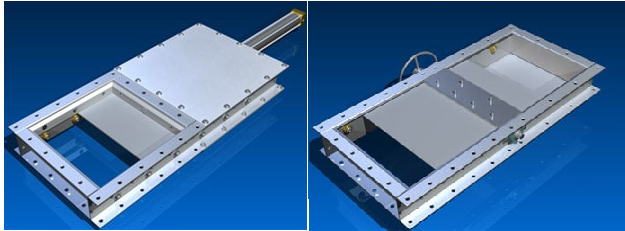
\includegraphics[scale=0.7]{img/slides.png}
			\end{center}
			\caption{Mecanismo de Compuerta Deslizante. Tomada de \cite{DEM} \label{deslis}}
		\end{figure} % Ponerle negrilla		
	\end{itemize}
	

\subsubsection{Leyes y Normatividad}  \label{leyes}
Requerida para que el avance ganadero se realice de manera coordinada o estandarizada basada en las buenas prácticas ganaderas en pro de mejorar la productividad y ayudarla a alcanzar niveles de ganadería bovina del mundo \cite{invima}. 
\begin{itemize}
	\item \textbf{Decreto 1500 de 2007:} Reglamento técnico a través del cual se crea el Sistema Oficial de Inspección, Vigilancia y Control de la Carne y otros productos comestibles y derivados cárnicos destinados para el consumo humano.
	\item \textbf{Decreto 072 de 2007:} Por el cual estable el manual de buenas prácticas de manejo para la producción de ganado bovino.
	\item \textbf{Decreto 2905 de 2007:} Por el cual se establece el reglamento técnico sobre los requisitos sanitarios y de inocuidad de la carne y productos cárnicos comestibles de las especies bovina y bufalina destinados para el consumo humano.
	\item \textbf{Decreto 18119 de 2007:} Por el cual se reglamenta los requisitos del plan gradual de cumplimiento para  las plantas de beneficio y desposte de bovino y bufalinos.
	\item \textbf{Decreto 2278 de 1982:} Reglamentación parcial en el titulo V de la ley 09 de 1979 que se refiere al sacrificio de animales de abasto público o para consumo humano y el procesamiento, transporte y comercialización de su carne.
\end{itemize}



\subsubsection{Conceptos adicionales}

\begin{itemize}

	\item \textbf{Algoritmos Computacionales:}
	Los algoritmos son un conjunto de instrucciones o reglas predefinidas de manera ordenada que permiten llevar a cabo una actividad mediante pasos consecutivos secuenciales o paralelos de manera no ambigua para poder realizar una actividad \cite{algoritmo}. Los algoritmos computacionales son algoritmos más sofisticados y precisos que permiten aprovechar las nuevas tecnolog\'ias y que al depender de una memoria finita deben ser lo mas optimizados posible para que puedan procesar grandes cantidades de datos con limitaciones finitas y generalmente a bajo costo. 

	\item \textbf{Almacenamiento en la nube:}
	 La nube, también denominada como ``Cloud Storage" (Ver Figura \ref{cloudpng}), se refiere tanto a las aplicaciones entregadas como servicios a través de internet y el sfotware del hardware y sistemas en los centros de datos que proporcionan estos servicios \cite{cloud2}.
	\begin{figure}[H]
	\begin{center}
		
\includegraphics[scale=0.35]{img/cloud.png}
	\end{center}
	\caption{Almacenamiento en nube. \label{cloudpng}}
	\end{figure}

	\item \textbf{Bases de datos digitales:}
	Es un conjunto de datos interrelacionados y almacenados de forma ordenada y sistem\'atica (Ver Figura \ref{databasepng}) para un uso posterior\cite{database}. Debido al desarrollo tecnol\'ogico de la inform\'atica y la electr\'onica, estas bases de datos suelen ser digitales y por lo general se almacenan en la nube (Cloud). Por otra parte, es considerado un modelo de almacenamiento de datos basado en redes de computadoras, donde los datos est\'an alojados en espacios de almacenamiento virtualizados \cite{cloud}.
	\begin{figure}[H]
		\begin{center}
			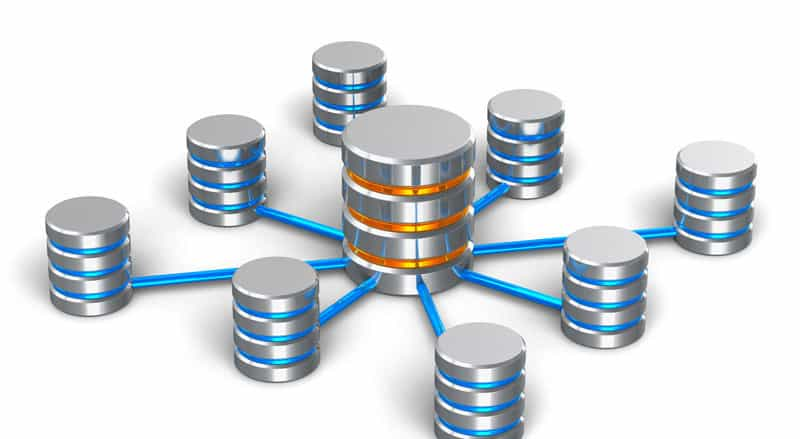
\includegraphics[scale=0.35]{img/databasepng.png}
		\end{center}
	\caption{Base de datos. \label{databasepng}}
	\end{figure}
	
	\item \textbf{Ganadería de carne:}
	 Es un ciclo productivo de cabezas de ganado destinadas al engorde que comprende un proceso prolongado en el tiempo que consta de varias etapas que abarcan desde el nacimiento vivo de la cría, siguiendo con su crecimiento y finalmente su comercialización en producto final, ya sea en carne, lácteos o sus derivados (Ver Figura \ref{ganadcarnepng}).
	 
	\begin{figure}[H]
	\begin{center}
		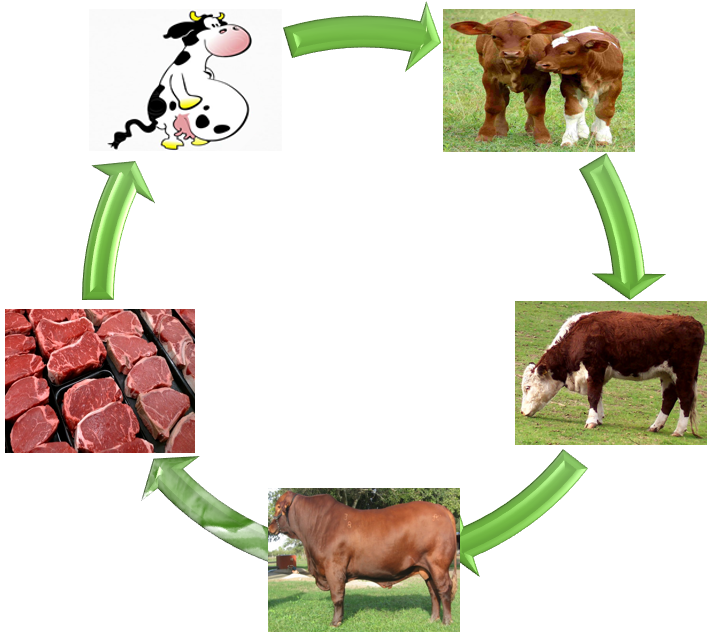
\includegraphics[scale=0.7]{img/ganadcarne.png}
	\end{center}
	\caption{Ganadería de carne. \label{ganadcarnepng}}
	\end{figure}
	
	\item \textbf{RFID:}
	 La identificación por radiofrecuencia (Ver Figura \ref{rfid1png}), es un sistema reprogramable de almacenamiento y recuperación de datos de manera inalámbrica mediante etiquetas, tarjetas o transpondedores en general, que pueden ser adheridas a productos, animales e incluso a personas sin necesidad de alimentación interna. Este sistema tiene una gran variedad de aplicaciones entre las cuales se pueden mencionar logísticas de distribución, servicios industriales, control de acceso, entre otros \cite{rfid1}.
	\begin{figure}[H]
	\begin{center}
		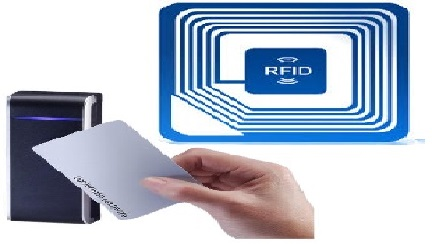
\includegraphics[scale=0.7]{img/rfid1.png}
	\end{center}
	\caption{Sistemas RFID. \label{rfid1png}}
	\end{figure}
	
\end{itemize}


%%%%%Debe incluir las referencias de manera adecuada, por ejemplo, \cite{cp-book}. (2-3 p\'aginas). Así mismo, los cuadros y figuras deben ser numeradas y referenciadas en el texto, por ejemplo, ver Figura \ref{escudo} y Cuadro \ref{tab:tabla-ejemplo}

%%%%%%%%%%%%%%%
% Figura de Ejemplo
%%%%%%%%%%%%%%%
%%\begin{figure}
%%	\begin{center}
%%		
\includegraphics{img/pujlogo.png}
%%	\end{center}
%%	\caption{Escudo Javeriana \label{escudo}}
%%\end{figure}

%%%%%%%%%%%%%%%
% Tabla de ejemplo
%%%%%%%%%%%%%%%

%%%\begin{table}
%%%\centering
%%%\begin{tabular}{ | l | l | l |}
%%%\hline
%%%{\bf Col 1} &{\bf  Col 2} & {\bf Col3} \\ \hline
%%%Fila 1 & Fila 2 & Fila 3 \\ \hline
%%%\end{tabular}
%%%\caption{Tabla de Ejemplo \label{tab:tabla-ejemplo}}
%%%\end{table}


\subsection{Trabajos Relacionados}
En esta área de trabajo se pueden encontrar innumerables trabajos de grado que usan al sector agroindustrial como oportunidad de desarrollo. Algunos de los trabajos previos y referentes al desarrollo de este trabajo de grado se pueden mencionar a los siguientes:

\begin{itemize}
\item \textbf{"Diseño, modelamiento y simulación de maquina dosificadora de alimento granulado para animales":} En este trabajo desarrollado por los estudiantes egresados de la Universidad de La Salle, Carlos Pinto y Hernán Durán, se puede  evidenciar el desarrollo tanto mecánico como electrónico de un dosificador giratorio de alimento granulada para aves.  El objetivo de este trabajo es facilitar el diseño de sistemas electrónicos que puedan ser implementados a nivel comercial, con la finalidad de  ayudar a incrementar el nivel productivo de las empresas ganaderas avícolas. En este proyecto se utilizó el modelamiento 3D como herramienta principal para el desarrollo del prototipo funcional usado para la dosificación del alimento granulado. El modelo final desarrollado se puede apreciar en la Figura \ref{lasal}:
			\begin{figure}[H]
			\begin{center}
			 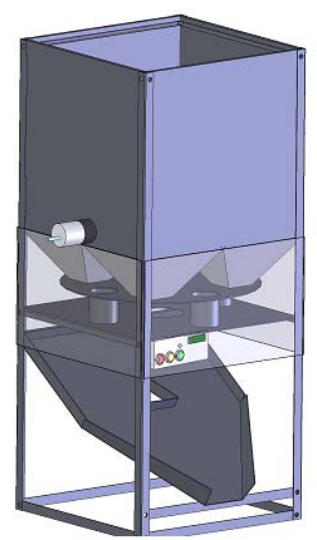
\includegraphics[scale=0.55]{img/lasal1png.png}
			\end{center}
			\caption{Unidad completa de dosificación. Tomada de \cite{pinturan} \label{lasal}}
			\end{figure}
			
\item \textbf{"Dispensador automático de comida para mascotas, programable y controlado remotamente":} Mediante este trabajado de grado, realizado por los Ingenieros Electrónicos de la Universidad del Valle John León y Daniel Rueda, se realiza el diseño y la implementación de un alimentador automático de mascotas que pueda ser controlador mediante una aplicación móvil para facilitar el uso y garantizar la dosificación del alimento al animal doméstico  en las horas que lo requiera \cite{univalle1}. Una característica similar al trabajo planteado es el uso de avisos y notificaciones móviles para los casos en los que el dispensador no cuente con suficiente alimento o que el dosificador no haya podido entregar el alimento correctamente.
Este sistema fue desarrollado mediante simulación e impresión 3D y la aplicación para la interfaz de usuario fue realizada mediante software Open Source para Android. El dispositivo final se puede apreciar en la Figura \ref{univalle1}:

			\begin{figure}[H]
			\begin{center}
			 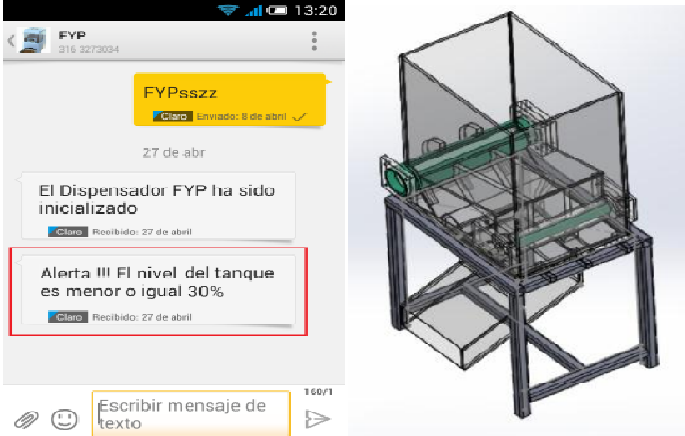
\includegraphics[scale=0.45]{img/univalle1png.png}
			\end{center}
			\caption{Unidad completa de dosificación. Tomada de \cite{univalle1} \label{univalle1}}
			\end{figure}			
			
\item \textbf{"Feedstar":} Este es un sistema automático de dosificación de alimento en grandes cantiadades especialmente diseñado para ahorrar espacio \cite{feedstar}. En la figura \ref{feedstar1} se observa una simulación del sistema, el cual puede ser regulado en tamaño y longitud y abastecer grandes cantidades de ganado mediante una correa extendible y un sistema de dosificación continuo que garantizan suministrar las grandes cantidades de alimento, minerales y forraje para abastecer ganado en sistemas de ganado estabulado. Este producto se encuentra a nivel comercial desarrollado por la empresa alemana EDER. 

			\begin{figure}[H]
			\begin{center}
			 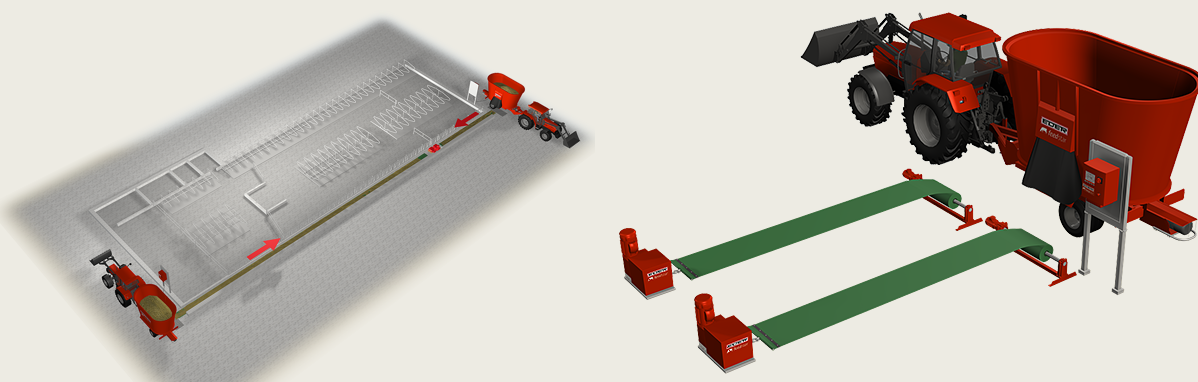
\includegraphics[scale=0.35]{img/feedstarpng.png}
			\end{center}
			\caption{Sistema Feedstar. Tomada de \cite{feedstar} \label{feedstar1}}
			\end{figure}	
			
			
\item \textbf{"Dosificador automático de alimento y agua para el ganado vacuno de la Finca Molina, en la comunidad de San Rafael del Sur":} Este es un trabajo de grado respaldado por la Universidad Autónoma de Nicaragua, que consiste en un sistema integral para suministrar alimento y agua a ganado vacuno en una finca de aproximadamente 7 hectáreas y el cual sería controlado mediante un PLC \cite{nicaraguat}. En este trabajo se plantea el diseño visto en la Figura \ref{nicaragua1} donde se puede observar el control de diferentes sensores para proveer correcta y eficientemente la dosificación de alimento y agua por cada cabeza de ganado ubicadas en sus respectivos cubículos perteneciente al sistema.

			\begin{figure}[H]
			\begin{center}
			 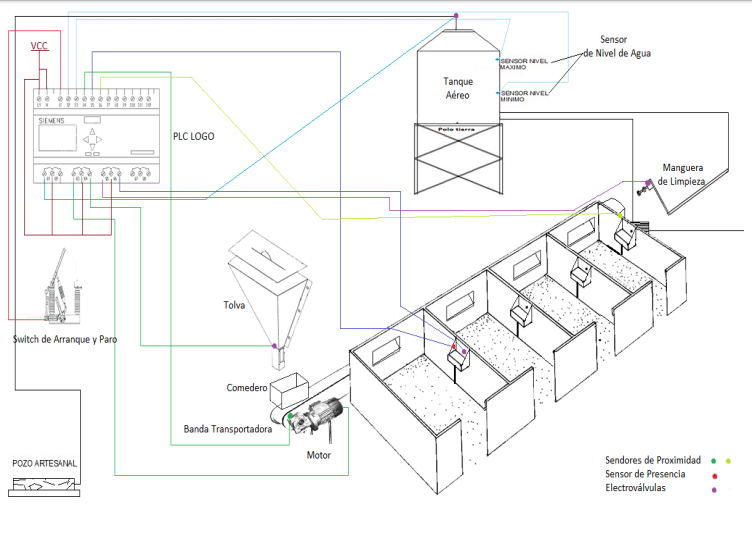
\includegraphics[scale=0.9]{img/nicaraguapng.png}
			\end{center}
			\caption{Sistema alimenticio de la Finca Molina. Tomada de \cite{nicaraguat} \label{nicaragua1}}
			\end{figure}	
			
			
\end{itemize}


\section{Metodolog\'ia}

\subsection{Tipo de Estudio y Metodolog\'ia a usar} 
%Definir y explicar el tipo de estudio (exploratorio, descriptivo, correlacional, explicativo).
Este proyecto, al igual que todo proceso de desarrollo, tiene un m\'etodo que caracteriza su evoluci\'on; por tal raz\'on se propone el uso de la metodolog\'ia CDIO como base metodol\'ogica para la realizaci\'on de este proyecto. 
Esta metodología  ha sido formada por las principales escuelas de Ingeniería de Estados Unidos, Europa, Canadá, Reino Unido, África, Asia y Nueva Zelanda; como una forma de colaboración a nivel mundial para desarrollar una nueva visión de enseñanza de la ingeniería.\\

Esta metodolog\'ia permite proporcionar las herramientas necesarias para desarrollar propuestas innovadoras a trav\'es de un an\'alisis sistem\'atico a partir de la problem\'atica planteada. y est\'a compuesta por 4 fases que consisten en Concebir, Diseñar, Implementar y Operar sistemas de ingeniería con valor agregado en un ambiente moderno para crear sistemas y productos. El proyecto ser\'a  dirigido y monitoreado por parte del director del proyecto semanalmente para verificar, controlar y corregir lo que se irá trabajando día a día por el estudiante a lo largo del proyecto.

\begin{itemize}
	\item \textbf{NOTA 1: Debido a los alcances mencionados en la secci\'on \ref{limites}, este proyecto no incluir\'a la fase de Implementaci\'on debido a que este es un proyecto de dise\~no. Mas sin embargo constará de una construcción de un prototipo para suplir la fase de Implementación y validar la fase de Operación.}
	\item \textbf{NOTA 2: La realizaci\'on de tareas no necesariamente es de manera secuencial y se encontrar\'an actividades que se realicen paralelamente}.\\\\
\end{itemize}

\subsection{Actividades} \label{actividades}
%\textbf{\textit{\Estas todavía no son las actividades es solo como para ver como quedaría una estructura parecida, ES soo un FORMATO}}
\begin{itemize}
\item[1)] Fase de Concepción:
	\begin{itemize}
	
	\item Identificaci\'on del área temática, normatividad, limitaciones técnicas y tecnológicas, usuarios; contextos sociales, culturales, ambientales y necesidades de la problem\'atica.
	\item Búsqueda bibliogr\'afica referente a la tem\'atica.
	\item Analizar trabajos previos y antecedentes para búsqueda de oportunidades o posibles mejoras.
	\item Investigaci\'on de posibles herramientas y dispositivos que aporten al desarrollo del trabajo de grado.
	\item Buscar, clasificar y seleccionar las herramientas y los dispositivos a utilizar.
	\item Establecer parámetros de entrada y salida (In/Out).

	\end{itemize}
	
\item[2)] Fase de Dise\~no:
	\begin{itemize}

	\item Dise\~nar el sistema de medici\'on y obtenci\'on de informaci\'on.
	\item Dise\~nar los algoritmos para cada dispositivo con base en los parámetros In/Out.
	\item Dise\~nar la identificación exitosa de cada animal por separado.
	\item Dise\~nar la verificación de alimento suficiente para dar abasto a las raciones del día.
	\item Dise\~nar el aviso o alarma en caso que no haya suficiente alimento para suplir las necesidades dietarias del día para los animales.
	\item Dise\~nar la dosificación del alimento y los mecanismos que se requieran para tal fin.
	\item Dise\~nar el pesaje de la ración dosificada que será suministrada a cada res de acuerdo con su dieta respectiva.
	\item Dise\~nar el suministro del alimento dosificado.
	\item Dise\~nar la verificación de que el alimento ha sido suministrado.
	\item Dise\~nar la verificación de que el alimento suministrado ha sido ingerido satisfactoriamente.
	\item Dise\~nar la verificación que permita corroborar si un animal ya ha sido alimentado en una franja horaria determinada para negar dosificaciones repetidas.
	\item Dise\~nar el aviso o la alarma en caso de presentarse un caso de negación por dosificación repetida.
	\item Dise\~nar el aviso al personal y registro en el historial de la res correspondiente en caso tal que no se ingiera el alimento
	\item Dise\~nar el proceso para la toma de peso de cada una de las reses en un grupo determinado. 
	\item Dise\~nar el registro de la información de manera automática.
	\item Dise\~nar la representaci\'on de la informaci\'on.
	\item Dise\~nar el prototipo del prototipo a escala para la prueba del concepto.
	\item Dise\~nar el plan de pruebas.
	
	\end{itemize}
	
\item[3)] Fase de Construcci\'on:

	\begin{itemize}
	
	\item Construcción del prototipo.
	\item Construcción del plan de pruebas.
	
	\end{itemize}
	
\item[4)] Fase de Operaci\'on:

	\begin{itemize}
	
	\item Verificaci\'on de la funcionalidad de los dispositivos.
	\item Verificaci\'on de la funcionalidad de los algoritmos.
	\item Verificación de los resultados para correcciones (si la hay) del plan de pruebas.
	\item Verificaci\'on de la funcionalidad del prototipo.
	\item Evaluaci\'on de los resultados.
	
	\end{itemize}

\item[5)] Otros:

	\begin{itemize}
	
	\item Reuniones de control con director del proyecto.
	\item Realización de la documentación del proyecto.
	
	\end{itemize}
\end{itemize}		

\section{Resultados Esperados}
% Hip\'otesis que se deben evaluar al final del proyecto (1 p\'agina)\\
 
 Los resultados esperados en este proyecto son:
 \begin{itemize}
 	\item Diseño de un sistema automático de alimentación de ganado de reses estabuladas en proceso de Ceba.
 	\item Identificar a cada individuo por separado mediante el sensor de RFID.
 	\item Dosificar exitosamente raciones de un gramaje acorde a la porción requerida para cada animal cultivado basado en su dieta preestablecida.
 	\item Tomar registro de la dosificación y entrega exitosa de alimento.
 	\item Verificar la cantidad de alimento racionado antes de ser depositado en la bandeja y tomar registro de ello.
 	\item Entregar el alimento racionado a cada individuo una única vez en una misma franja horaria y tomar registro de ello.
 	\item Dar aviso si se presenta un caso de intento de repetición de ración dosificada en una misma franja horaria por un mismo animal.
 	\item Verificar que el animal haya ingerido su porción, tomar registro de ello y dar aviso en caso contrario. 	
 	\item Obtener el peso del animal y tomar registro de ello.
 	\item Verificar que se tenga alimento suficiente para suministrar las porciones del día y dar aviso oportuno en caso contrario.
 	\item Hacer registro en la nube de los datos registrados por cada sensor.
 	\item Dar aviso de observaciones predefinidas por el productor de ceba mediante avisos y/o alarmas.
 	\item Mostrar los datos evolutivamente mediante ayudas gráficas.
 	\item Prototipo físico (a escala) del sistema diseñado con un solo dosificador funcional.
 	\item El diseño del prototipo y del sistema total posibilite hasta 4 dosificadores completamente funcionales.
 	\item Plan de pruebas.%\\ \\ \\ \\ \\ \\ \\ \\ \\ \\ \\ \\ \\ \\ \\ \\ \\ \\ \\ \\ \\ \\ \\ \\ \\ \\    
 \end{itemize} 
% 
\section{Cronograma}
%%%El cronograma por semana incluyendo las actividades descritas en la Secci\'on \ref{actividades}. 
En el Cuadro \ref{cronograma}, se evidencian las actividades previamente mencionadas en la sección \ref{actividades}, las cuales se realizar\'an para el desarrollo del proyecto.
%\\ \\ \\ \\ \\
% \ref{cronograma}.
 
%%%\begin{table}[H]
%%%	\begin{center}
%%%		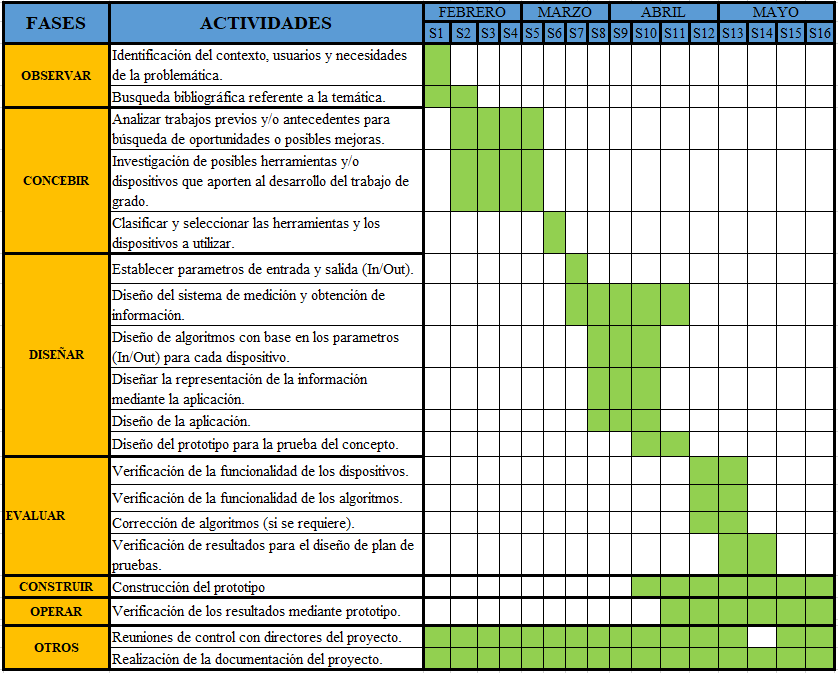
\includegraphics[scale=0.8]{img/cronopng4_5.png} %este comienzxa en febrero por als correciones de alexander
%%%	\end{center}
%%%	\caption{Cronograma del proyecto. \label{cronograma}}
%%%\end{table}
\begin{table}%[H]

\begin{ganttchart}[ 
x unit = 0.22cm, 
y unit chart = 0.4 cm,
y unit title = 0.45 cm,
milestone label font=\tiny,
group label font=\small,
title label font=\tiny,
%bar label font=\tiny,
time slot format=isodate, 
time slot format/start date=2015-03-25,
progress=today,
%time slot unit=week,
%canvas/.append style={fill=none, draw=black!60 , line width=.75pt},  %Este es el cuadrado blanco "La hoja" por así decrilo donde estan las barras del diagrama de gantt, esta sin fill y con bordes (yo creo que un 60 eta bien) y el grosor esta bien
hgrid,% style/.style={draw=none, line width=0pt}, % Esta es una linea que esta debajo del titulo  (Cronograma de actividades en este caso)
vgrid,%={*1{draw=black!40, line width=.5pt}}, % Estas son las lineas verticales del Diagrama de gantt, es mejor dejarlas delgadas y claras
%today=1,%\today,
today={\the\year-\the\month-\the\day},
today rule/.style={draw=black!90,dash pattern=on 3.0pt off 4.5pt,line width=1.2pt},
today label font=\small\bfseries,
%title/.style={draw=none, fill=none},%%%%%%%%%%%%%%%%%%%%%%%%%%%%%%%%%%%%%%%%%%%%%%%%%%%%%%%%%%%
%%%title label font=\bfseries\footnotesize,
%%%title label node/.append style={below=0pt}, % esto es que tan separado del titulo estan Marzo, Abril y Mayo
%%%include title in canvas=true, % hace llegar el recuadro de la cuadricula hasta por encima del titulo y se veo feo SI ESTA EN TRUE
bar label font=\mdseries\tiny\color{black!85}, % esto afecta la tonalidad de las palabras ACTIVIDAD 1.2.3.....
%%%%%bar label node/.append style={align=left,left=1cm}, % Separación entre las actividades y la cuadricula con las barras de gantt
bar label node/.append style={left=0.1cm},
bar/.append style={draw=none, fill=bargreen}, % ESTE NUMERO CAMBIA LA TONALIDAD DEL LA BARRA que va completando la tarea
%  EN UN PORCENTAJE DE NEGRO DEL 1-100
bar incomplete/.append style={fill=barblue}, % cambia la barra de fondo que es la que se debe completar en el porcentaje de avance
bar progress label font=\mdseries\tiny\color{black!99}, % Cambia la tonalidad del Porcentaje -> ejemplo ==== 10% completado
bar progress label node/.append style={below left=-6pt and -33pt},
bar label node/.append style={below left=-7pt and 0pt},%que tan hacia arriba o abajo aparece el letrero Activity
%%% de Finish to start y que tan hacia la derecha o izquierda aparece
group incomplete/.append style={fill=black!15}, % esta es la barra  del avance total del cronograma
group progress label font=\mdseries\small\color{black!99}, %footnotesize
group progress label node/.append style={below left=-6pt and -33pt},
group label node/.append style={below left=6pt and 0pt},
%%group left shift=0,
%%group right shift=0,
group height=0.4, % Esto es que tan alta es la barra grande del avance neto del proyecto
group peaks tip position=0,
group label node/.append style={left=0.1cm},
group/.append style={draw=none, fill=groupgreen}, % ESTE NUMERO CAMBIA LA TONALIDAD DEL LA BARRA que va completando la tarea
group progress label font=\bfseries\tiny,
%%link/.style={-latex, line width=1.5pt, linkred},
%%link label font=\scriptsize\bfseries,
%%link label node/.append style={below left=-2pt and 0pt},%que tan hacia arriba o abajo aparece el letrero
%%% de Finish to start y que tan hacia la derecha o izquierda aparece
]
%{1}{10}
{2019-03-25}{2019-05-30}
%{2019/03/25}{2019/05/30}
%\gantttitlecalendar{year, month=shortname, week, day} \\
\gantttitlecalendar{year, month=name, week} \\
%\gantttitlecalendar*[compress calendar,time slot format=isodate]{2019-03-22}{2019-05-30}{year, month} \\
%\gantttitlecalendar*[compress calendar,time slot format=isodate]{2015-11-1}{2018-10-30}{year, month} \\


%\ganttbar[bar/.append style={fill=blue}]{Goal Document}{2015-03-02}{2015-03-20}\\ 

%%%%\gantttitle{CRONOGRAMA DE ACTIVIDADES}{10} \\[grid]
%\gantttitle{CRONOGRAMA DE ACTIVIDADES}{10} \\[grid]
%\gantttitle{Marzo}{2}
%\gantttitle{Abril}{4}
%\gantttitle{Mayo}{4}\\
%\gantttitle[title label node/.append style={below left=-1pt and 15pt}]{Semana N.o:}{0} 
% Esto es la posicion hacia abajo de lo que dice Semana N.o 1
%\gantttitlelist{1,...,10}{1} \\

\ganttgroup{THESIS}{2019-03-25}{2019-05-30} \\
%\ganttgroup{THESIS}{2019/03/25}{2019/05/30} \\
%\ganttgroup[progress=20]{TESIS}{1}{10} \\
%%%
\ganttgroup{CONCEIVE}{2019-03-25}{2019-05-03} \\
%\ganttgroup{CONCEIVE}{2019/03/25}{2019/05/03} \\
%%%\ganttgroup[progress=65]{CONCEBIR}{1}{6} \\
%%%
\ganttbar[name=bar1]{\textbf{Activity 1}}{2019-03-25}{2019-03-30} \\
%\ganttbar[name=bar1]{\textbf{Activity 1}}{2019/03/25}{2019/03/30} \\
%%%\ganttbar[progress=100,name=bar1]{\textbf{Activity 1}}{1}{1} \\
%%%
\ganttbar[name=bar2]{\textbf{Activity 2}}{2019-03-25}{2019-03-30} \\
%\ganttbar[name=bar2]{\textbf{Activity 2}}{2019/03/25}{2019/03/30} \\
%%%\ganttbar[progress=14,name=bar2]{\textbf{Activity 2}}{1}{1} \\
%%%
\ganttbar[name=bar3]{\textbf{Activity 3}}{2019-03-25}{2019-03-30} \\
%\ganttbar[name=bar3]{\textbf{Activity 3}}{2019/03/25}{2019/03/30} \\
%%%\ganttbar[progress=25,name=bar3]{\textbf{Activity 3}}{1}{1} \\
%%%
\ganttbar[name=bar4]{Activity 4}{2019-03-25}{2019-03-30} \\
%\ganttbar[name=bar4]{Activity 4}{2019/03/25}{2019/03/30} \\

%%%\ganttbar[progress=56,name=bar4]{Activity 4}{1}{1} \\
%%%
\ganttbar[name=bar5]{\textbf{Activity 5}}{2019-03-25}{2019-04-30} \\
%\ganttbar[name=bar5]{\textbf{Activity 5}}{2019/03/25}{2019/04/30} \\
%%%\ganttbar[progress=100,name=bar5]{\textbf{Activity 5}}{1}{6} \\
%%%
\ganttbar[name=bar6]{\textbf{Activity 6}}{2019-03-25}{2019-04-30} \\
%\ganttbar[name=bar6]{\textbf{Activity 6}}{2019/03/25}{2019/04/30} \\
%%%\ganttbar[progress=100,name=bar6]{\textbf{Activity 6}}{1}{6} \\
%%%
\ganttgroup{DESIGN}{2019-04-01}{2019-05-18} \\
%\ganttgroup{DESIGN}{2019/04/01}{2019/05/18} \\
%%%\ganttgroup[progress=30]{DISEÑAR}{2}{8} \\
%%%
\ganttbar[name=bar7]{\textbf{Activity 7}}{2019-04-01}{2019-05-05} \\
%\ganttbar[name=bar7]{\textbf{Activity 7}}{2019/04/01}{2019/05/05} \\
%%%\ganttbar[progress=14,name=bar7]{\textbf{Activity 7}}{2}{6} \\
%%%
\ganttbar[name=bar8]{\textbf{Activity 8}}{2019-04-01}{2019-05-05} \\
%\ganttbar[name=bar8]{\textbf{Activity 8}}{2019/04/01}{2019/05/05} \\
%%%\ganttbar[progress=25,name=bar8]{\textbf{Activity 8}}{2}{6} \\
%%%
\ganttbar[name=bar9]{\textbf{Activity 9}}{2019-04-01}{2019-04-14} \\
%\ganttbar[name=bar9]{\textbf{Activity 9}}{2019/04/01}{2019/04/14} \\
%%%\ganttbar[progress=56,name=bar9]{\textbf{Activity 9}}{2}{3} \\
%%%
\ganttbar[name=bar10]{\textbf{Activity 10}}{2019-04-01}{2019-04-14} \\
%\ganttbar[name=bar10]{\textbf{Activity 10}}{2019/04/01}{2019/04/14} \\
%%%\ganttbar[progress=100,name=bar10]{\textbf{Activity 10}}{2}{3} \\
%%%
\ganttbar[name=bar11]{\textbf{Activity 11}}{2019-04-01}{2019-04-21} \\
%\ganttbar[name=bar11]{\textbf{Activity 11}}{2019/04/01}{2019/04/21} \\
%%%\ganttbar[progress=100,name=bar11]{\textbf{Activity 11}}{2}{4} \\
%%%
\ganttbar[name=bar12]{\textbf{Activity 12}}{2019-04-01}{2019-04-21} \\
%\ganttbar[name=bar12]{\textbf{Activity 12}}{2019/04/01}{2019/04/21} \\
%%%\ganttbar[progress=14,name=bar12]{\textbf{Activity 12}}{2}{4} \\
%%%
\ganttbar[name=bar13]{\textbf{Activity 13}}{2019-04-08}{2019-04-14} \\
%\ganttbar[name=bar13]{\textbf{Activity 13}}{2019/04/08}{2019/04/14} \\
%%%\ganttbar[progress=25,name=bar13]{\textbf{Activity 13}}{3}{3} \\
%%%
\ganttbar[name=bar14]{\textbf{Activity 14}}{2019-04-15}{2019-04-21} \\
%\ganttbar[name=bar14]{\textbf{Activity 14}}{2019/04/15}{2019/04/21} \\
%%%\ganttbar[progress=56,name=bar14]{\textbf{Activity 14}}{4}{4} \\
%%%
\ganttbar[name=bar15]{\textbf{Activity 15}}{2019-04-15}{2019-04-21} \\
%\ganttbar[name=bar15]{\textbf{Activity 15}}{2019/04/15}{2019/04/21} \\
%%%\ganttbar[progress=20,name=bar15]{\textbf{Activity 15}}{4}{4} \\
%%%
\ganttbar[name=bar16]{\textbf{Activity 16}}{2019-04-15}{2019-04-21} \\
%\ganttbar[name=bar16]{\textbf{Activity 16}}{2019/04/15}{2019/04/21} \\
%%%\ganttbar[progress=30,name=bar16]{\textbf{Activity 16}}{4}{4} \\
%%%
\ganttbar[name=bar17]{\textbf{Activity 17}}{2019-04-01}{2019-04-14} \\
%\ganttbar[name=bar17]{\textbf{Activity 17}}{2019/04/01}{2019/04/14} \\
%%%\ganttbar[progress=14,name=bar17]{\textbf{Activity 17}}{2}{3} \\
%%%
\ganttbar[name=bar18]{\textbf{Activity 18}}{2019-04-01}{2019-04-21} \\
%\ganttbar[name=bar18]{\textbf{Activity 18}}{2019/04/01}{2019/04/21} \\
%%%\ganttbar[progress=25,name=bar18]{\textbf{Activity 18}}{2}{4} \\
%%%
\ganttbar[name=bar19]{\textbf{Activity 19}}{2019-04-01}{2019-04-21} \\
%\ganttbar[name=bar19]{\textbf{Activity 19}}{2019/04/01}{2019/04/21} \\
%%%\ganttbar[progress=56,name=bar19]{\textbf{Activity 19}}{2}{4} \\
%%%
\ganttbar[name=bar20]{\textbf{Activity 20}}{2019-04-08}{2019-04-28} \\
%\ganttbar[name=bar20]{\textbf{Activity 20}}{2019/04/08}{2019/04/28} \\
%%%\ganttbar[progress=20,name=bar20]{\textbf{Activity 20}}{3}{5} \\
%%%
\ganttbar[name=bar21]{\textbf{Activity 21}}{2019-04-08}{2019-05-5} \\
%\ganttbar[name=bar21]{\textbf{Activity 21}}{2019/04/08}{2019/05/5} \\
%%%\ganttbar[progress=10,name=bar21]{\textbf{Activity 21}}{3}{6} \\
%%%
\ganttbar[name=bar22]{\textbf{Activity 22}}{2019-04-22}{2019-05-12} \\
%\ganttbar[name=bar22]{\textbf{Activity 22}}{2019/04/22}{2019/05/12} \\
%%%\ganttbar[progress=14,name=bar22]{\textbf{Activity 22}}{5}{7} \\
%%%
\ganttbar[name=bar23]{\textbf{Activity 23}}{2019-04-15}{2019-05-12} \\
%\ganttbar[name=bar23]{\textbf{Activity 23}}{2019/04/15}{2019/05/12} \\
%%%\ganttbar[progress=25,name=bar23]{\textbf{Activity 23}}{4}{7} \\
%%%
\ganttbar[name=bar24]{\textbf{Activity 24}}{2019-04-01}{2019-05-19} \\
%\ganttbar[name=bar24]{\textbf{Activity 24}}{2019/04/01}{2019/05/19} \\
%%%\ganttbar[progress=56,name=bar24]{\textbf{Activity 24}}{2}{8} \\
%%%
\ganttgroup{CONSTRUCT}{2019-04-1}{2019-05-19} \\
%\ganttgroup{CONSTRUCT}{2019/04/1}{2019/05/19} \\
%%%\ganttgroup[progress=30]{CONSTRUIR}{2}{8} \\
%%%
\ganttbar[name=bar25]{\textbf{Activity 25}}{2019-04-22}{2019-05-19} \\
%\ganttbar[name=bar25]{\textbf{Activity 25}}{2019/04/22}{2019/05/19} \\
%%%\ganttbar[progress=10,name=bar25]{\textbf{Activity 25}}{5}{8} \\
%%%
\ganttbar[name=bar26]{\textbf{Activity 26}}{2019-04-22}{2019-05-19} \\
%\ganttbar[name=bar26]{\textbf{Activity 26}}{2019/04/22}{2019/05/19} \\
%%%\ganttbar[progress=10,name=bar26]{\textbf{Activity 26}}{5}{8} \\
%%%
\ganttgroup{OPERATE}{2019-04-15}{2019-05-30} \\
%\ganttgroup{OPERATE}{2019/04/15}{2019/05/30} \\
%%%\ganttgroup[progress=30]{OPERAR}{4}{10} \\
%%%
\ganttbar[name=bar27]{\textbf{Activity 27}}{2019-05-06}{2019-05-26} \\
%\ganttbar[name=bar27]{\textbf{Activity 27}}{2019/05/06}{2019/05/26} \\
%%%\ganttbar[progress=14,name=bar27]{\textbf{Activity 27}}{7}{9} \\
%%%
\ganttbar[name=bar28]{\textbf{Activity 28}}{2019-05-06}{2019-05-26} \\
%\ganttbar[name=bar28]{\textbf{Activity 28}}{2019/0506}{2019/05/26} \\
%%%\ganttbar[progress=25,name=bar28]{\textbf{Activity 28}}{7}{9} \\
%%%
\ganttbar[name=bar29]{\textbf{Activity 29}}{2019-05-06}{2019-05-26} \\
%\ganttbar[name=bar29]{\textbf{Activity 29}}{2019/05/06}{2019/05/26} \\
%%%\ganttbar[progress=56,name=bar29]{\textbf{Activity 29}}{7}{9} \\
%%%
\ganttbar[name=bar30]{\textbf{Activity 30}}{2019-05-13}{2019-05-30} \\
%\ganttbar[name=bar30]{\textbf{Activity 30}}{2019/05/13}{2019/05/30} \\
%%%\ganttbar[progress=56,name=bar30]{\textbf{Activity 30}}{8}{9.5} \\
%%%
\ganttbar[name=bar31]{\textbf{Activity 31}}{2019-05-13}{2019-05-30} \\
%\ganttbar[name=bar31]{\textbf{Activity 31}}{2019/05/13}{2019/05/30} \\
%%%\ganttbar[progress=56,name=bar31]{\textbf{Activity 31}}{8}{10} \\
%%%
\ganttgroup{OTHERS}{2019-03-25}{2019-05-30} \\
%\ganttgroup{OTHERS}{2019-03-25}{2019-05-30} \\
%%%\ganttgroup[progress=30]{OTROS}{1}{10} \\
%%%
\ganttbar[name=bar32]{\textbf{Activity 32}}{2019-03-25}{2019-05-30} \\
%\ganttbar[name=bar32]{\textbf{Activity 32}}{2019/03/25}{2019/05/30} \\
%%%\ganttbar[progress=56,name=bar32]{\textbf{Activity 32}}{1}{10} \\
%%%
\ganttbar[name=bar33]{\textbf{Activity 33}}{2019-03-25}{2019-05-30}
%\ganttbar[name=bar33]{\textbf{Activity 33}}{2019/03/25}{2019/05/30}
%%%\ganttbar[progress=56,name=bar33]{\textbf{Activity 33}}{1}{10} \\
%

%\ganttmilestone{Hito 1}{11}{11}  \\
%\ganttmilestone{Hito 2}{12}{12} \\
%\ganttbar[progress=35,]{\textbf{Activity 8}}{12}{22} \\
%\ganttbar[progress=0,]{\textbf{Activity 9}}{23}{24} \\
%\ganttmilestone{Q6 report}{9}{10} \\
%\ganttmilestone{M2: Project finished}{5}{10}


%%%\ganttlink[link type=f-s]{bar1}{bar2}
%%%\ganttlink[link type=f-s]{bar4}{bar5}


\end{ganttchart}
\caption{Cronograma del proyecto. \label{cronograma}}
\end{table}
%\end{tikzpicture}


%\end{document}


\section{Recursos}

\subsection{Humanos}
\subsubsection{Director}
\begin{itemize}
\item El ingeniero Electr\'onico, Eugenio Tamura. Curs\'o su pregrado en la Universidad del Cauca.
Obtuvo su Maestr\'ia y Doctorado en Arquitectura y Tecnolog\'ia de los Sistemas Inform\'aticos, en la Universidad Polit\'ecnica de Valencia, Espa\~na.\\
Actualmente es Director de Carrera de Ingenier\'ia Electr\'onica  y profesor de Pregrado, Maestr\'ia y Doctorado.

\end{itemize} 
\subsubsection{Estudiante}
El estudiante de Ingenier\'ia Electr\'onica  \authorA, llevar\'a a cabo el desarrollo de este proyecto para optar por el título de Ingeniero Electrónico en la Pontificia Universidad Javeriana Cali.


%%%%%%%%%%%%%%%
% Tabla de ejemplo
%%%%%%%%%%%%%%%

%%%\begin{table}
%%%\centering
%%%\begin{tabular}{ | l | l | l |}
%%%\hline
%%%{\bf Col 1} &{\bf  Col 2} & {\bf Col3} \\ \hline
%%%Fila 1 & Fila 2 & Fila 3 \\ \hline
%%%\end{tabular}
%%%\caption{Tabla de Ejemplo \label{tab:tabla-ejemplo}}
%%%\end{table}


\subsection{Econ\'omicos}
\subsubsection{Consideraciones}
El desarrollo de este proyecto requerir\'a establecer lo siguiente:


\begin{itemize}

	\item Consideraciones del proyecto respecto a la Universidad visto en el cuadro \ref{tabconsidPUJ}:
	
\begin{table}[H]
\centering
\scalebox{0.8}{
{\setlength{\arrayrulewidth}{0.8mm}
\begin{tabular}{ | >{\columncolor{tabla1}} p{3.8cm} | p{0.45cm} | >{\columncolor{tabla1}} p{3.0cm} | p{2.1cm} | >{\columncolor{tabla1}} p{3.5cm} | p{4cm} | }
\hline
{\bf\centering \bfseries\small Director(es)} & {\bf\centering  1} & {\bf\centering \bfseries\small Salario Mensual por Director \\ (Aproximado).}
 & {\bf\centering \bfseries\small \$ 7'.000.000} & {\bf\centering \bfseries\small Cantidad total de horas por  semana} & {\bf\centering  2}\\ \hline
{\bf\centering \bfseries\small \# Días trabajados al mes} & {\bf\centering   20} & {\bf\centering \bfseries\small Horas trabajadas al día} & {\bf\centering   8}
 & {\bf\centering \bfseries\small  Frecuencia de atención y dirección (semanal)} & {\bf\centering  1-2}\\ \hline
{\bf\centering \bfseries\small \# Horas de dirección por sesión } & {\bf\centering  2.5} & {\bf\centering \bfseries\small Costo Hora Director} & {\bf \bfseries\small \$ 43.750} & {\bf\centering \bfseries\small  Equipos de trabajo} & {\bf\centering  \bfseries\small Propios de la Universidad}\\ \hline
{\bf\centering \bfseries\small  \# Total de Horas dedicadas al proyecto.} & {\bf  25} & {\bf\centering  \bfseries\small Costo Total Horas Trabajo de Dirección} & {\bf\centering \bfseries\small  \$ 1'.093.750} & {\bf\centering \bfseries\small  Software  adicional} & {\bf\centering \bfseries\small  Licencias  y Software educativo a nombre de la Universidad}\\ \hline
\end{tabular}}}
\caption{Consideraciones del proyecto respecto a la Pontificia Universidad Javeriana \label{tabconsidPUJ}}
\end{table}	

%%\begin{table}
%%\centering
%%\resizebox{10cm}{!} {
%%\begin{tabular}{|c|c|c|c|c|c|c|c|c|}
%%\hline
%%\multicolumn{5}{|c|}{Puerto fuente} & \multicolumn{4}{|c|}{Puerto destino} \\ \hline
%%\multicolumn{}{|c|}{Numero de secuencia} \\ \hline
%%\multicolumn{9}{|c|}{Numero de reconocimiento} \\ \hline
%%Longitud cabecera & Reservado & URG & ACK & PSH & RST & SYN & FIN & Tamaño ventana \\ \hline
%%\multicolumn{5}{|c|}{Suma verificación} & \multicolumn{4}{|c|}{Puntero a datos urgentes} \\ \hline
%%\multicolumn{9}{|c|}{Opciones} \\ \hline
%%\multicolumn{9}{|c|}{Datos} \\ \hline
%%\end{tabular}
%%}
%%\caption{Estructura de un segmento TCP.}
%%\label{c2_tabla_segento_tcp}
%%\end{table}





	
	
	
%%%	\begin{table}[H]
%%%		\begin{center}
%%%			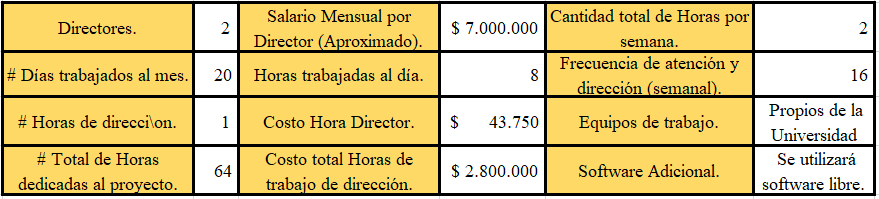
\includegraphics[scale=0.8]{img/considPUJ.png}
%%%		\end{center}
%%%		\caption{Consideraciones del proyecto respecto a la universidad. \label{tabconsidPUJ}}	
%%%	\end{table}
	
	\item Consideraciones del proyecto respecto al estudiante visto en el cuadro \ref{tabconsidYo}:
	
\begin{table}[H]
\centering
\scalebox{0.7}{
{\setlength{\arrayrulewidth}{0.8mm}
\begin{tabular}{ | >{\columncolor{tabla2}} p{3cm} | p{1.2cm} | >{\columncolor{tabla2}} p{3.5cm} | p{2.2cm} | >{\columncolor{tabla2}} p{4cm} | p{2.5cm} | }
\hline
{\bf\centering \bfseries\small Estudiante(s)} & {\bf\centering  1} & {\bf\centering \bfseries\small Salario Mensual por Estudiante \\ (Aproximado).}
 & {\bf\centering \bfseries\small \$ 1'.300.000} & {\bf\centering \bfseries\small Cantidad total de horas por  semana} & {\bf\centering  60}\\ \hline
{\bf\centering \bfseries\small  \# Total de Horas dedicadas al proyecto} & {\bf\centering 600} & {\bf\centering \bfseries\small \# Horas trabajadas al día} & {\bf\centering   10}
 & {\bf\centering \bfseries\small  \# Total de semanas trabajadas} & {\bf\centering  10}\\ \hline
 {\bf\centering \bfseries\small  \# Costo hora Estudiante} & {\bf\centering \$ 5.417} & {\bf\centering \bfseries\small Costo total Horas de trabajo dedicadas al proyecto} & {\bf \bfseries\small \$ 4'.160.000} & {\bf\centering \bfseries\small Equipos, Software y material de trabajo adicional} & {\bf\centering  Propios del estudiante} \\ \hline
\end{tabular}}}
		\caption{Consideraciones del proyecto respecto al estudiante. \label{tabconsidYo}}
\end{table}		
	
	
	
%	\begin{table}[H]
%		\begin{center}
%			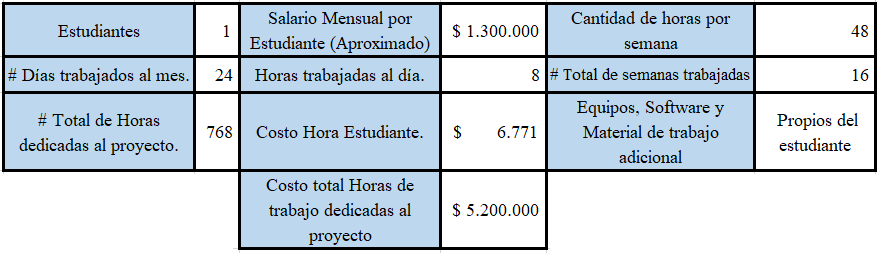
\includegraphics[scale=0.8]{img/considYo.png}
%		\end{center}
%		\caption{Consideraciones del proyecto respecto al estudiante. \label{tabconsidYo}}
%	\end{table}

\end{itemize}       


\subsubsection{Presupuesto}
El presupuesto del proyecto se observa en el Cuadro \ref{tabpresupuesto}.%
%	

%%%\begin{table}[H]
%%%\centering
%%%\scalebox{0.7}{
%%%{\setlength{\arrayrulewidth}{0.8mm}
%%%\begin{tabular}{ | p{1cm} | p{3cm} | p{5cm} |  p{2.5cm} | p{3.5cm} | p{3cm} | }
%%%\hline
%%%\begin{sideways}\multirow{5}{*}{UNIVERSIDAD}\end{sideways} & \multicolumn{1}{|>{\columncolor{blue2}}|}{CONCEPTO} & \multicolumn{1}{|>{\columncolor{blue2}}|}{REFERENCIA} & \multicolumn{1}{|>{\columncolor{blue2}}|}{CANT.} & \multicolumn{1}{|>{\columncolor{blue2}}|}{\$/Unidad} & \multicolumn{1}{|>{\columncolor{blue2}}|}{SUB TOTAL}\\ 
%%%\cline{2-6}
%%% & \multicolumn{1}{|>{\columncolor{tabla2}}|}{Costos dirección de trabajo de grado} & \multicolumn{1}{|>{\columncolor{beige}}|}{Asesoría y dirección del trabajo de grado del estudiante} & \multicolumn{1}{|>{\columncolor{beige}}|}{1} & \multicolumn{1}{|>{\columncolor{beige}}|}{\$ 546.875} & \multicolumn{1}{|>{\columncolor{beige}}|}{\$ 546.875}\\
%%%\cline{2-6}
%%% & \multicolumn{1}{|>{\columncolor{tabla2}}|}{Seguridad social y costos adicionales} & \multicolumn{1}{|>{\columncolor{beige}}|}{Costos adicionales por contratación de personal del proyecto} & \multicolumn{1}{|>{\columncolor{beige}}|}{1} & \multicolumn{1}{|>{\columncolor{beige}}|}{\$ 109.375} & \multicolumn{1}{|>{\columncolor{beige}}|}{\$ 109.375}\\
%%%\cline{2-6}
%%% & \multicolumn{1}{|>{\columncolor{tabla2}}|}{Equipos o instrumentación adicional} & \multicolumn{1}{|>{\columncolor{beige}}|}{Costo aproximado de sensores, elementos, herramientas, servicios y material de trabajo} & \multicolumn{1}{|>{\columncolor{beige}}|}{1} & \multicolumn{1}{|>{\columncolor{beige}}|}{\$ 2'.000.000} & \multicolumn{1}{|>{\columncolor{beige}}|}{\$ 2'000.000}\\
%%%\cline{2-6}
%%%%
%%%%
%%% & \multicolumn{4}{|>{\columncolor{lightgreen}}|}{SUBTOTAL} & \multicolumn{1}{|>{\columncolor{lightgreen}}|}{\$ 2'.656.250}\\
%%%\hline
%%%%
%%%%\begin{sideways}\multirow{5}{|>{\columncolor{darkgreen}}c|}{Estudiante}\end{sideways} & \multicolumn{1}{|>{\columncolor{blue2}}c|}{Concepto} & \multicolumn{1}{|>{\columncolor{blue2}}c|}{Referencia} & \multicolumn{1}{|>{\columncolor{blue2}}c|}{Cant.} & \multicolumn{1}{|>{\columncolor{blue2}}c|}{\$\/Unidad} & \multicolumn{1}{|>{\columncolor{blue2}}c|}{Subtotal 1}\\
%%%%%\cline{}
%%%%& & \multicolumn{1}{|>{\columncolor{tabla2}}c|}{Costos de trabajo por estudiante practicante} & \multicolumn{1}{|>{\columncolor{beige}}c|}{Investigación, Mano de obra y desarrollo del trabajo de grado del estudiante} & \multicolumn{1}{|>{\columncolor{beige}}c|}{1} & \multicolumn{1}{|>{\columncolor{beige}}c|}{3'.250.000} & \multicolumn{1}{|>{\columncolor{beige}}c|}{3'.250.000}\\
%%%%& & \multicolumn{1}{|>{\columncolor{tabla2}}c|}{Seguridad social y costos adicionales} & \multicolumn{1}{|>{\columncolor{beige}}c|}{Costos adicionales por contratación de personal estudiantil del proyecto} & \multicolumn{1}{|>{\columncolor{beige}}c|}{1} & \multicolumn{1}{|>{\columncolor{beige}}c|}{650.000} & \multicolumn{1}{|>{\columncolor{beige}}c|}{650.000}\\
%%%%& & \multicolumn{1}{|>{\columncolor{tabla2}}c|}{Equipos o instrumentación adicional} & \multicolumn{1}{|>{\columncolor{beige}}c|}{Costo aproximado de sensores, elementos, servicios, software y\/o material de trabajo} & \multicolumn{1}{|>{\columncolor{beige}}c|}{1} & \multicolumn{1}{|>{\columncolor{beige}}c|}{1'.000.000} & \multicolumn{1}{|>{\columncolor{beige}}c|}{1'.000.000}\\
%%%%
%%%%& & \multicolumn{4}{|>{\columncolor{lightgreen}}c|}{SUBTOTAL} & \multicolumn{1}{|>{\columncolor{lightgreen}}c|}{4'.900.000}\\
%%%%
%%%%\multicolumn{5}{|>{\columncolor{darkgreen}}c|}{COSTOS TOTALES} & \multicolumn{1}{|>{\columncolor{darkgreen}}c|}{7'.556.250}
%%%
%%%\end{tabular}}}
%%%		\caption{Presupuesto del proyecto. \label{tabconsidYo}}
%%%\end{table}		
%%%	


%%\begin{tabular}{|l|l|l|l|}\hline
%%  %\multirow{5}{*}{numeric literals} & \multirow{5}{*}{integers} & in decimal & \verb|8743| \\ \cline{3-4}
%%  \multirow{5}{*}{UNIVERSIDAD} & \multicolumn{1}{|l|}{CONCEPTO} & \multicolumn{1}{|l|}{REFERENCIA} & \multicolumn{1}{|l|}{CANT.} & \multicolumn{1}{|l|}{\$/Unidad} & \multicolumn{1}{|l|}{SUB TOTAL}\\
%%  & & \multirow{2}{*}{in octal} & \verb|0o7464| \\ \cline{4-4}
%%  & & & \verb|0O103| \\ \cline{3-4}
%%  & & \multirow{2}{*}{in hexadecimal} & \verb|0x5A0FF| \\ \cline{4-4}
%%  & & & \verb|0xE0F2| \\ \cline{2-4}
%%  & \multirow{5}{*}{fractionals} & \multirow{5}{*}{in decimal} & \verb|140.58| \\ \cline{4-4}
%%  & & & \verb|8.04e7| \\ \cline{4-4}
%%  & & & \verb|0.347E+12| \\ \cline{4-4}
%%  & & & \verb|5.47E-12| \\ \cline{4-4}
%%  & & & \verb|47e22| \\ \cline{1-4}
%%  \multicolumn{3}{|l|}{\multirow{3}{*}{char literals}} & \verb|'H'| \\ \cline{4-4}
%%  \multicolumn{3}{|l|}{} & \verb|'\n'| \\ \cline{4-4}          %% here
%%  \multicolumn{3}{|l|}{} & \verb|'\x65'| \\ \cline{1-4}        %% here
%%  \multicolumn{3}{|l|}{\multirow{2}{*}{string literals}} & \verb|"bom dia"| \\ \cline{4-4}
%%  \multicolumn{3}{|l|}{} & \verb|"ouro preto\nmg"| \\ \cline{1-4}          %% here
%%\end{tabular}



	\begin{table}[H]
		\begin{center}
			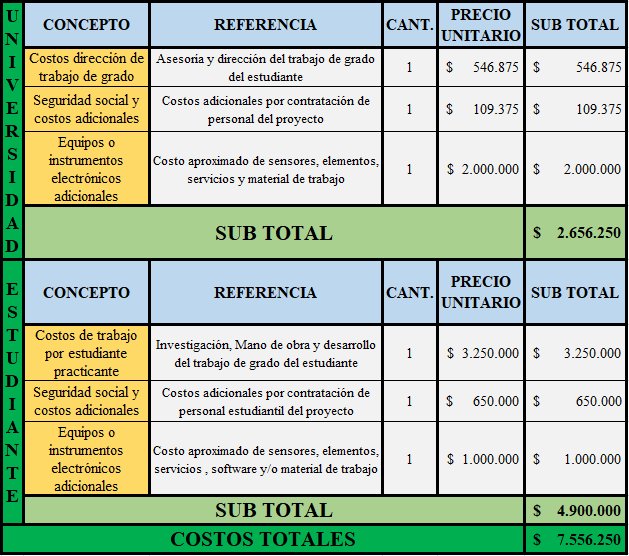
\includegraphics[scale=0.9]{img/presuTot3.png}
		\end{center}
		\caption{Presupuesto del proyecto. \label{tabpresupuesto}}
	\end{table}

 


%\chapter*{Anexos} \label{anexus}
% %A continuación se presentan los anexos del proyecto:
%\begin{itemize}
%	\item Consideraciones para presupuesto del proyecto:
		\begin{figure}
			\begin{center}
				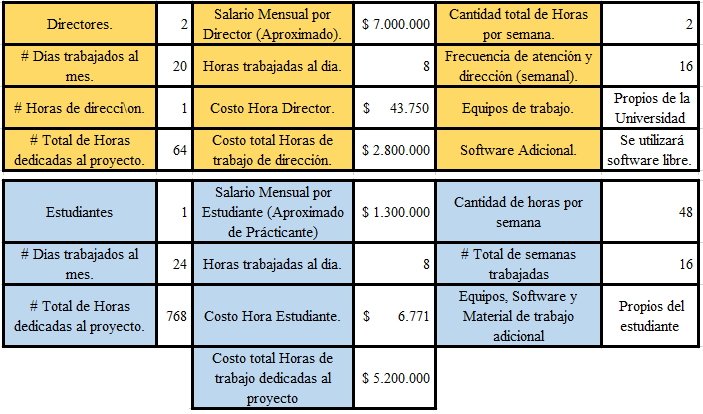
\includegraphics{img/consideraciones2.png}
			\end{center}
			\caption{Consideraciones para el presupuesto \label{tabconsideraciones}}
		\end{figure}
%	\item Presupuesto del proyecto:
		\begin{figure}
			\begin{center}
				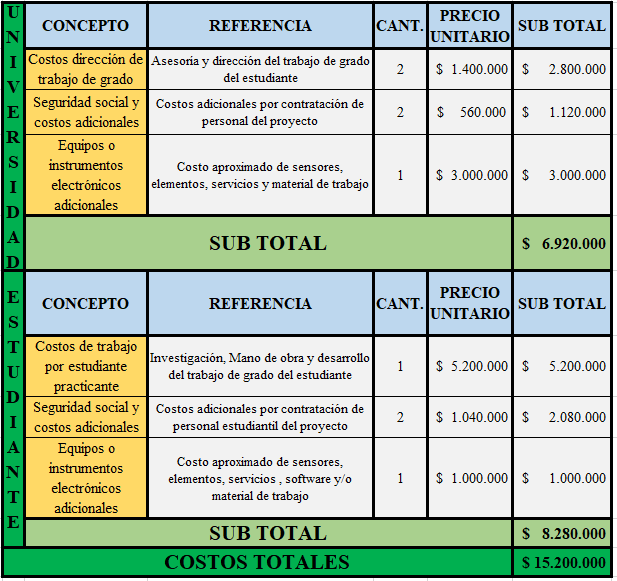
\includegraphics{img/presuTot.png}
			\end{center}
			\caption{Presupuesto \label{tabpresupuesto}}
		\end{figure}
%	\item Cronograma del proyecto:
		\begin{figure}
			\begin{center}
				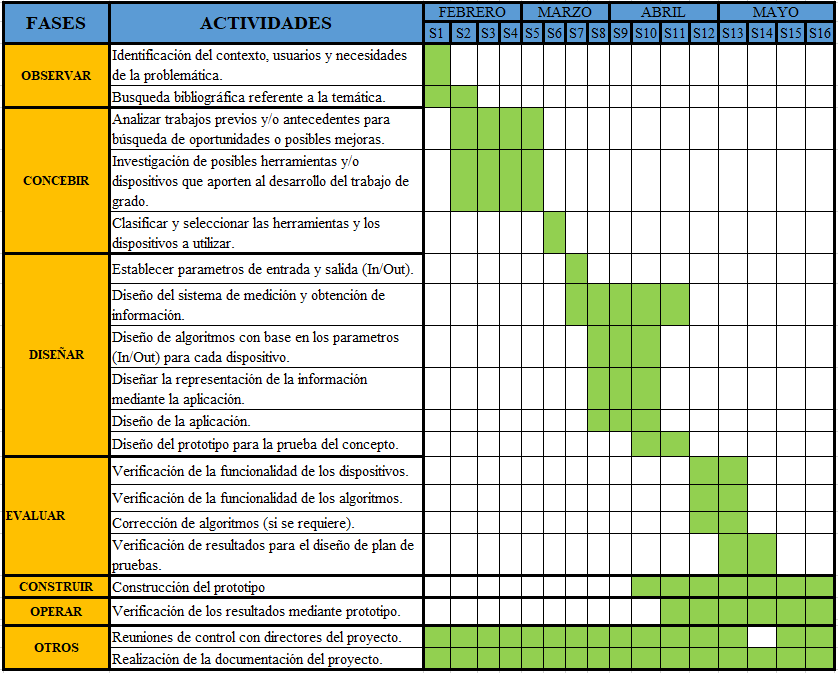
\includegraphics{img/cronopng4_5.png}
%				\includegraphics{img/cronopng2.png} %este es el que tiene colores mas oscuro po si no se ve bien el otro
			\end{center}
			\caption{Cronograma del proyecto. \label{cronograma}}
		\end{figure}
%\end{itemize} 



%%%%%%%%%%%%%%%%%%%%%%%%%%%%%
% BIBLIOGRAFIA
%%%%%%%%%%%%%%%%%%%%%%%%%%%%%

\bibliographystyle{plain}
\bibliography{docs/biblio}

%%%%%%%%%%%%%%%%
% GENERAL INDEX
%%%%%%%%%%%%%%%%

\printindex

\end{document}

%\endinput
